 %%%%%%%%%%%%%%%%%%%%%%%%%%%%%%%%%%%%%%%%%%
%                                        %
% Szablon pracy dyplomowej inżynierskiej % 
%                                        %
%%%%%%%%%%%%%%%%%%%%%%%%%%%%%%%%%%%%%%%%%%



\documentclass[a4paper,twoside,12pt]{book}
\usepackage[utf8]{inputenc}                                      
\usepackage[T1]{fontenc}  
\usepackage{amsmath,amsfonts,amssymb,amsthm}
\usepackage[british,polish]{babel}
\addto\captionspolish{\renewcommand{\figurename}{Rys.}}
\usepackage{siunitx}

\usepackage{indentfirst}
\usepackage{lmodern}
\usepackage{graphicx}
\usepackage[hidelinks]{hyperref} 
\usepackage{booktabs}
%\usepackage{tikz}
%\usepackage{pgfplots}
\usepackage{mathtools}
\usepackage{geometry}
\usepackage[page]{appendix} % toc,
\renewcommand{\appendixtocname}{Dodatki}
\renewcommand{\appendixpagename}{Dodatki}
\renewcommand{\appendixname}{Dodatek}
\usepackage{setspace}
\usepackage{float}
\usepackage{caption}
\usepackage{subcaption}
\usepackage{eurosym}
\onehalfspacing
\usepackage{graphicx}
\usepackage[backend=biber]{biblatex}

\addbibresource{Bibliografia/bibliografia.bib}


\frenchspacing

\usepackage{listings}
\lstset{
	language={},
	basicstyle=\ttfamily,
	keywordstyle=\lst@ifdisplaystyle\color{blue}\fi,
	commentstyle=\color{gray}
}

%%%%%%%%%

%%%% TODO LIST GENERATOR %%%%%%%%%

%\usepackage{tikz}
%\usepackage{manfnt}   % dangerous sign 
\usepackage{color}
\definecolor{brickred}      {cmyk}{0   , 0.89, 0.94, 0.28}

\makeatletter \newcommand \kslistofremarks{\section*{Uwagi} \@starttoc{rks}}
  \newcommand\l@uwagas[2]
    {\par\noindent \textbf{#2:} %\parbox{10cm}
{#1}\par} \makeatother


\newcommand{\ksremark}[1]{%
{%\marginpar{\textdbend}
{\color{brickred}{[#1]}}}%
\addcontentsline{rks}{uwagas}{\protect{#1}}%
}

\newcommand{\comma}{\ksremark{przecinek}}
\newcommand{\nocomma}{\ksremark{bez przecinka}}
\newcommand{\styl}{\ksremark{styl}}
\newcommand{\ortografia}{\ksremark{ortografia}}
\newcommand{\fleksja}{\ksremark{fleksja}}
\newcommand{\pauza}{\ksremark{pauza `--', nie dywiz `-'}}
\newcommand{\kolokwializm}{\ksremark{kolokwializm}}

%%%%%%%%%%%%%% END OF TODO LIST GENERATOR %%%%%%%%%%%

%%%%%%%%%%%% ZYWA PAGINA %%%%%%%%%%%%%%%
% brak kapitalizacji zywej paginy
\usepackage{fancyhdr}
\pagestyle{fancy}
\fancyhf{}
\fancyhead[LO]{\nouppercase{\it\rightmark}}
\fancyhead[RE]{\nouppercase{\it\leftmark}}
\fancyhead[LE,RO]{\it\thepage}


\fancypagestyle{tylkoNumeryStron}{%
   \fancyhf{} 
   \fancyhead[LE,RO]{\it\thepage}
}

\fancypagestyle{NumeryStronNazwyRozdzialow}{%
   \fancyhf{} 
   \fancyhead[LO]{\nouppercase{\it\rightmark}}
   \fancyhead[RE]{\nouppercase{\it\leftmark}}
   \fancyhead[LE,RO]{\it\thepage}
}


%%%%%%%%%%%%% OBCE WTRETY  
\newcommand{\obcy}[1]{\emph{#1}}
\newcommand{\angver}[1]{{\selectlanguage{british}\obcy{#1}}}
%%%%%%%%%%%%%%%%%%%%%%%%%%%%%

% polskie oznaczenia funkcji matematycznych
\renewcommand{\tan}{\operatorname {tg}}
\renewcommand{\log}{\operatorname {lg}}

% jeszcze jakies drobiazgi

\newcounter{stronyPozaNumeracja}

\newcommand{\hcancel}[1]{%
    \tikz[baseline=(tocancel.base)]{
        \node[inner sep=0pt,outer sep=0pt] (tocancel) {#1};
        \draw[red] (tocancel.south west) -- (tocancel.north east);
    }%
}%

\newcommand{\miesiac}{%
  \ifcase\the\month
  \or styczeń% 1
  \or luty% 2
  \or marzec% 3
  \or kwiecień% 4
  \or maj% 5
  \or czerwiec% 6
  \or lipiec% 7
  \or sierpień% 8
  \or wrzesień% 9
  \or październik% 10
  \or listopad% 11
  \or grudzień% 12
  \fi}


%%%%%%%%%%%%%%%%%%%%%%%%%%%%%%%%%%%%%%%%%%%%%%
% Helvetica font macros for the title page:
\newcommand{\headerfont}{\fontfamily{phv}\fontsize{18}{18}\bfseries\scshape\selectfont}
\newcommand{\titlefont}{\fontfamily{phv}\fontsize{18}{18}\selectfont}
\newcommand{\otherfont}{\fontfamily{phv}\fontsize{14}{14}\selectfont}

%%%%%%%%%%%%%%%%%%%%%%%%%%%%%%%%%%%%%%%%%%%%%%
%%%%%%%%%%%%%%%%%%%%%%%%%%%%%%%%%%%%%%%%%%%%%%
%%%%%%%%%%%%%%%%%%%%%%%%%%%%%%%%%%%%%%%%%%%%%%
%%%%%%%%%%%%%%%%%%%%%%%%%%%%%%%%%%%%%%%%%%%%%%
%%%%%%%%%%%%%%%%%%%%%%%%%%%%%%%%%%%%%%%%%%%%%%
%%%%%%%%%%%%%%%%%%%%%%%%%%%%%%%%%%%%%%%%%%%%%%
%%%%%%%%%%%%%%%%%%%%%%%%%%%%%%%%%%%%%%%%%%%%%%


\newcommand{\autor}{Rafał Osadnik}
\newcommand{\promotor}{dr hab. Tomasz Błachowicz, Prof. PŚ}
\newcommand{\tytul}{Rekonstrukcja i analiza stanu nieważkości w warunkach laboratoryjnych z użyciem klinostatu}
\newcommand{\polsl}{Politechnika Śląska}
\newcommand{\wydzial}{Instytut Fizyki}
\newcommand{\kierunek}{Kierunek: Fizyka Techniczna}
\begin{document}

%\kslistofremarks 
	
%%%%%%%%%%%%%%%%%%  STRONA TYTULOWA %%%%%%%%%%%%%%%%%%%
\pagestyle{empty}
{
	\newgeometry{top=2.5cm,%
	             bottom=2.5cm,%
	             left=3cm,
	             right=2.5cm}
	\sffamily
	\rule{0cm}{0cm}
	
	\begin{center}
	
\includegraphics[width=45mm]{logo.jpg}
	\end{center} 
	\vspace{1cm}
	\begin{center}
	\headerfont \polsl
	\end{center}
	\begin{center}
	\headerfont \wydzial
	\end{center}
	\begin{center}
	\headerfont \kierunek
	\end{center}
	\vfill
	\begin{center}
	\titlefont Praca dyplomowa inżynierska
	\end{center}
	\vfill
	
	\begin{center}
	\otherfont \tytul\par
	\end{center}
	
	\vfill
	
	\vfill
	 
	\noindent\vbox
	{
		\hbox{\otherfont Autor: \autor}
		\vspace{12pt}
		\hbox{\otherfont Promotor: \promotor}
		\vspace{12pt}
	}
	\vfill 
 
   \begin{center}
   \otherfont Gliwice,  \miesiac\ \the\year
   \end{center}	
	\restoregeometry
}
  

\cleardoublepage
 

\rmfamily
\normalfont



%%%%%%%%%%%%%%%%%% SPIS TRESCI %%%%%%%%%%%%%%%%%%%%%%
\pagenumbering{Roman}
\pagestyle{tylkoNumeryStron}
\tableofcontents

%%%%%%%%%%%%%%%%%%%%%%%%%%%%%%%%%%%%%%%%%%%%%%%%%%%%%
\setcounter{stronyPozaNumeracja}{\value{page}}
\mainmatter

\pagestyle{empty}


\chapter*{Streszczenie}

Na świecie obecnie obserwuje się gwałtowny rozwój przemysłu kosmicznego. Z każdym kolejnym rokiem kwota inwestowana w firmy tego sektora zwiększa się, osiągając poziom 9.1 miliarda dolarów w roku 2020. Szacuje się, iż ta kwota zostanie przekroczona pod koniec obecnego 2021-go roku. Tak gwałtowny wzrost nieuchronnie doprowadzi do sytuacji, w których koniecznością będzie również wysyłanie coraz większej liczby ludzi w kosmos. To naturalnie zrodzi zapotrzebowanie na technologię produkcji przedmiotów i materiałów niezbędnych do życia, w warunkach pozaziemskich, ze względu na wysokie koszty wynoszenia ładunku poza Ziemię (mała pojemność kapsuł transportowych). Warunki pozaziemskie tj. o niskiej grawitacji bądź mikrograwitacji, dla biologicznych struktur wzrostowych np. roślin, można symulować na Ziemi za pomocą specjalnych urządzeń - klinostatów. Pozwala to na badanie wpływu warunków panujących w kosmosie na owe struktury bez konieczności wynoszenia ich na orbitę, co znacznie redukuje koszty badań.  

Celem obecnej pracy jest rozwój projektu budowy i wykonania klinostatu, którego podstawową koncepcję wykonano w ramach projektu Project Based Learning (PBL), w którym uczestniczyłem dwa lata temu. W czasie realizacji projektu klinostatu zaprojektowano wiele autorskich usprawnień mechanicznych, które również zostały opisane w tej pracy. Główną częścią pracy dyplomowej jest projekt i wykonanie systemu kontroli klinostatu, który pozwala dowolnemu użytkownikowi na łatwe i intuicyjne sterowanie tym urządzeniem. Cały system składa się z trzech modułów - sterownika kontrolera klinostatu, aplikacji pulpitowej oraz programu komputera komory uprawnej, służącego do akwizycji danych i przekazywania ich do aplikacji za pomocą łącza bezprzewodowego. Program komputera komory oraz aplikację pulpitową napisano w języku Python z wykorzystaniem popularnych bibliotek numerycznych (scipy) oraz tworzenia interfejsu (Tkinter). Sterownik klinostatu ze względu na implementację na platformie ze znacznie ograniczoną mocą obliczeniową oraz ograniczonymi zasobami zaprogramowano w języku C++. 

W początkowych rozdziałach pracy skupię się na podstawowych informacjach na temat klinostatów. Ma to na celu wprowadzenie czytającego w zasadę działania, konstrukcję oraz podział klinostatów, jak i przedstawienie obecnego stanu badań z ich wykorzystaniem. 

{\bf Słowa kluczowe:} klinostat, mikrograwitacja, oprogramowanie, wzrost, rośliny

\addcontentsline{toc}{chapter}{Streszczenie}



\cleardoublepage

\pagestyle{NumeryStronNazwyRozdzialow}
%%%%%%%%%%%%%% wlasciwa tresc pracy %%%%%%%%%%%%%%%%%


\chapter{Wstęp}

\section{Grawitotropizm}

\section{Klinostat}

\section{Zasada działania klinostatu}

\section{Rodzaje klinostatów}

\section{Obecne rozwiązania}

\graphicspath{{./PBL/images}}

\chapter{Udział w projekcie PBL}

Uczenie poprzez realizację projektów (ang. \angver{Project Based Learning}, PBL) jest metodą przyswajania wiedzy oraz nabywania kompetencji przez studentów poprzez rozwiązywanie rzeczywistych problemów. Dzięki takiemu podejściu, nowe informacje są zapamiętywane na zasadzie ich implementacji w rzeczywistości oraz daje to okazję do aplikacji już wcześniej zdobytej wiedzy i umiejętności. Pozwala to na głębsze zrozumienie treści oraz rozwój innych umiejętności takich jak krytyczne myślenie, praca w grupie i umiejętności komunikacyjne \cite{bib:PBL}. Rozdział ten poświęcony jest takiemu projektowi, w którym brałem udział dwa lata temu. Jego tematyką było zaprojektowanie układu laboratoryjnego przeznaczonego do badań nad wzrostem struktur biologicznych w warunkach mikrograwitacji z wyłączeniem ziemskiego pola magnetycznego. Moje subiektywne odczucia odnośnie tej metody nauki są bardzo pozytywne. Jestem pewien iż dzięki temu projektowi nauczyłem się znacznie więcej niż w przypadku konwencjonalnych metod nauczania. Nabyłem wiele umiejętności praktycznych np. metody tworzenia symulacji opartych o obliczenia równoległe, projektowanie elementów mechanicznych, tworzenie zapotrzebowań na części i surowce oraz wiele innych, które przydały się później \linebreak w osobistych projektach, praktykach czy też pracy zawodowej.

\section{Cel projektu} \label{cel_projektu}

Celem wspomnianego projektu było zaprojektowanie układu laboratoryjnego, składającego się z
 klatki Helmholtza oraz umieszczonego wewnątrz klinostatu trójwymiarowego. Docelowo taki układ
  pozwalałby na przeprowadzanie badań nad rozwojem roślin w warunkach symulowanej
   mikrograwitacji bez ziemskiego pola magnetycznego. Klatka Helmholtza jest złożeniem trzech
    par cewek Helmholtza \linebreak w takiej konfiguracji, aby osie magnetyczne każdej z par było
     prostopadłe do pozostałych. Pozwala to wytworzyć wektor indukjcji magnetycznej o dowolnym
      kierunku przestrzennym i bardzo wysokiej jednorodności. Wizualizację wyników \linebreak z przeprowadzonych symulacji można zobaczyć na Rys. \ref{fig:polemag} . Wysoka jednorodność jest kluczowa
       aby generowany wektor indukcji magnetycznej był stały \linebreak w objętości przeprowadzanego,
        eksperymentu. W związku z wymaganiami projektu, wewnętrzna konstrukcja klinostatu
         musiała zostać wykonana tak, aby mieć jak najmniejszy wpływ na panujące wewnątrz
          warunki magnetyczne. Naturalnie rodzi to zagadnienie wyboru materiałów konstrukcyjnych
           klinostatu, które nie powinny mieć właściwości ferromagnetycznych, powinny mieć
            względnie niską przewodność elektryczną w celu eliminacji indukowanych prądów
             wirowych oraz dodatkowym ich atutem będzie niska podatność magnetyczna. Oprócz
              właściwości magnetycznych materiałów istnotne są też możliwości ich obróbki
               termicznej oraz mechanicznej, a również ich forma, co później ma wpływ na
                prostotę montażu urządzenia. Oprócz samych wymagań materiałowych oraz
                 konstrukcyjnych, należało również zapewnić optymalne warunki wzrostowe obiektów
                  badawczych, należało określić odpowiedni rozmiar cewek, aby objętość o wysokim
                   stopniu jednorodności magnetycznej była odpowiednio duża oraz wiele innych.
                    Taki szereg wymagań stworzył bardzo ciekawe i multidyscyplinarne wyzwanie
                     inżynieryjne, które wymagało użycia oraz w niektórych przypadkach
                      stworzenia wielu środowisk symulacyjnych \linebreak w celu jego rozwiązania. Projekt
                       wykonywany był w zespole 5-cio osobowym \linebreak na przestrzeni jednego semestru.
                        Powstały na rzecz projektu model komputerowy układu klinostatu wraz z
                         klatką Helmholtza przedstawiony został na Rys.
                          \ref{fig:klatka_helmholtza}.
                          
                                
  \begin{figure}[t]
         	\centering
         	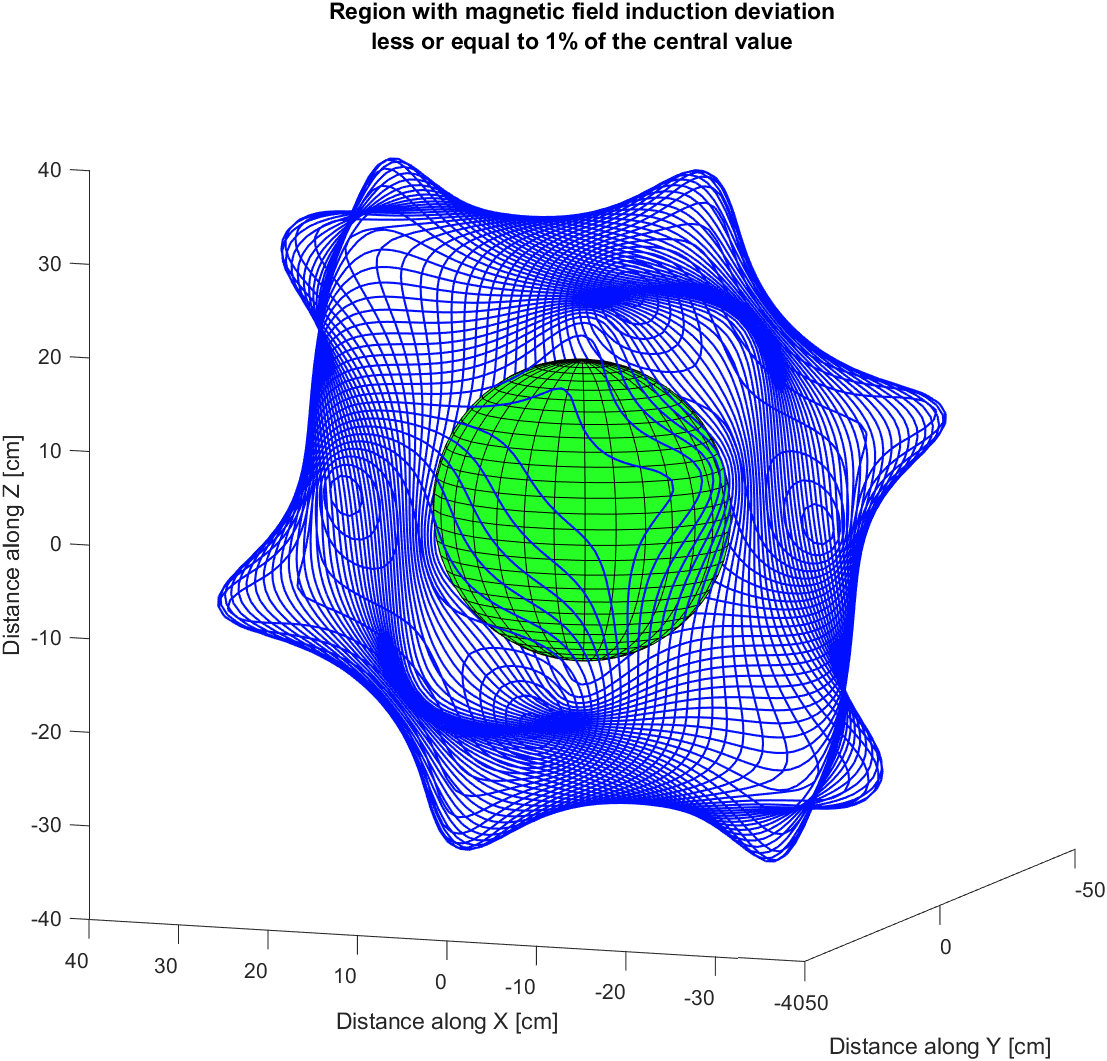
\includegraphics[scale=0.22]{pole_mag}
         	\caption{Wizualizacja objętości w której spełniony jest założony warunek jednorodności pola magnetycznego. Maksymalny odchyłek spełniający założenie przyjęto za 1\% wartości centralnej. Zielona sfera reprezentuje komorę środowiskową wybraną na jej podstawie. Źródło: [opracowanie własne].} 
         	\label{fig:polemag}
  \end{figure}
  

\begin{figure}
	\centering
	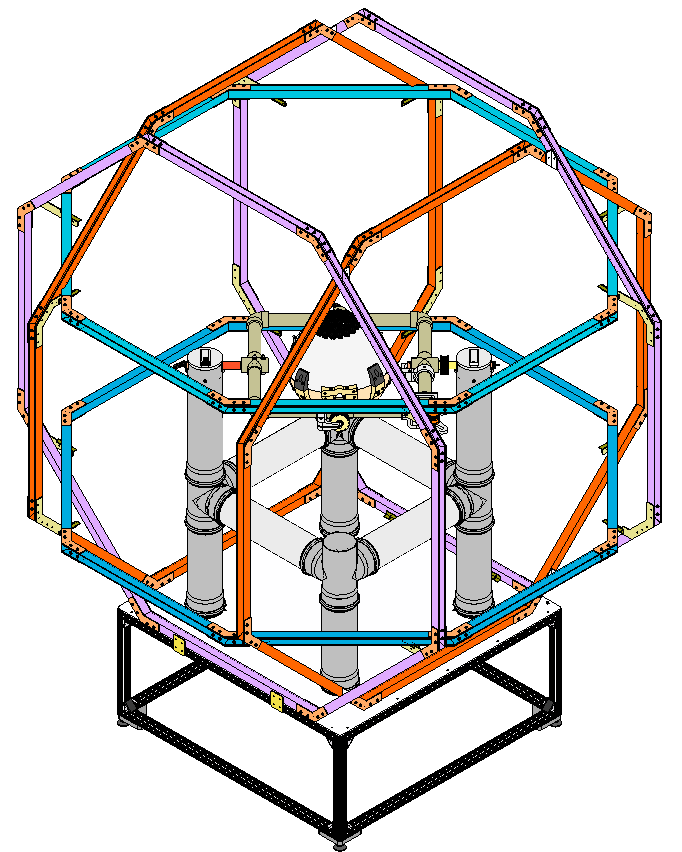
\includegraphics[scale=0.3]{klinostat_klatka}
	\caption{Projekt klatki Helmholtza z klinostatem. Źródło: [opracowanie własne].} 
	\label{fig:klatka_helmholtza}
\end{figure}

\section{Konstrukcja klinostatu} \label{konstrukcja}

Ten podrozdział poświęcony został krótkiemu opisowi konstrukcji samego klinostatu
zaprojektowanego w ramach PBL. Zaprojektowane urządzenie jest klinostatem o dwóch stopniach
swobody, każdy stopień posiada swój osobny napęd. Oznacza to iż jest to maszyna RPM, natomiast
jest możliwość uruchomienia go w trybach klinostatu 2-D oraz 3-D jak opisano w podrozdziale
\ref{klinostat3d}. Zewnętrzna rama klinostatu wykonana została z rur polipropylenowych (PP)
stabilizowanych włóknem szklanym. Odcinki rur wraz z kształtkami 90$^\circ$ oraz
czwórnikami zostały połączone metodą polifuzji termicznej (zgrzewanie). Tego typu rury
wykorzystywane są w instalacjach centralnego ogrzewania, dzięki czemu ich koszt jest
niski. Konstrukcję ramy przedstawiono na Rys. \ref{fig:rama_klinostatu}.Przeprowadzone
analizy elementów skończonych (FEM), wskazały iż materiał ten posiada wystarczającą
wytrzymałość, aby wykorzystać go jako element strukturalny ramy klinostatu. Jako wał
obrotowy wykorzystano rurę aluminiową o średnicy \SI{12}{mm}. Wykorzystanie
konwencjonalnych łożysk kulowych w konstrukcji klinostatu nie było wskazane ze
względu na wymagania opisane w podrozdziale \ref{cel_projektu}. Z tego powodu każdy
z interfejsów obrotowych stanowią tuleje ślizgowe wykonane z materiału
iglidur$\copyright$, zaprojektowanego przez firmę IGUS. Większość pozostałych
elementów została wykonana \linebreak w technologii druku przestrzennego z materiału PETG.
Konstrukcję jednego \linebreak z czterech czwórników ramy przedstawiono na Rys.
\ref{fig:czwórnik}. Wewnętrzny stopień swobody składa się z kulistej komory
środowiskowej, która posiada swój dedykowany komputer o niskiej mocy,
monitorujący panujące wewnątrz warunki oraz sterujący oświetleniem.
Zasilanie do wnętrza komory doprowadzone jest przez szereg złącz
ślizgowych, a przewody poprowadzone są wewnątrz ramy klinostatu. Podobne
rozwiązanie wykorzystano w obwodzie doprowadzjącym wodę, przewody
prowadzone są wewnątrz ramy klinostatu, a przy elementach obrotowych
zastosowano kolanka obrotowe. Rozmiar komory oraz typ i moc oświetlenia
zostały wyznaczone na podstawie wyników symulacji stworzonych na rzecz
projektu. Jej projekt przedstawiony został na Rys. \ref{fig:komora}.
Mocowania śrubowe zostały w większości zrealizowane za pomocą śrub
poliamidowych (PA). Komora została zaprojektowana tak, aby umożliwić operatorowi dostęp do jej
wnętrza bez konieczności jej demontażu \linebreak z ramy klinostatu.

\begin{figure}[]
	\centering
	
	\begin{subfigure}[b]{.49\textwidth}
		\centering
		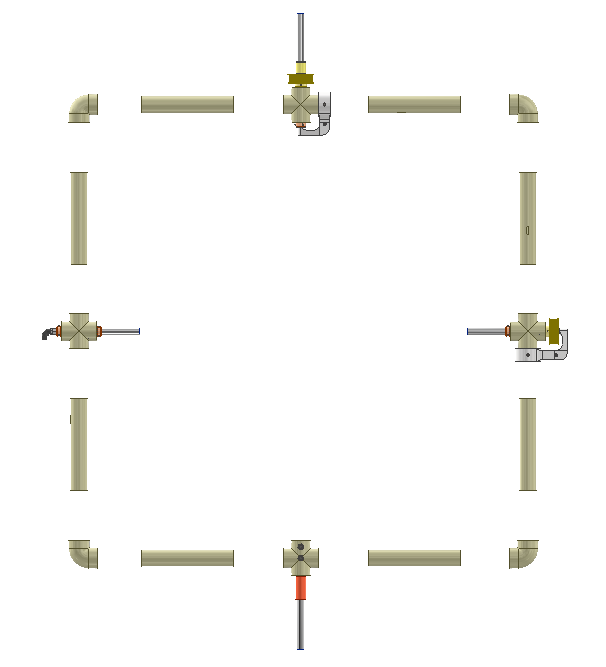
\includegraphics[width=\textwidth]{rama_40_aisass}
		\caption{Rama klinostatu.} 
		\label{fig:rama_klinostatu}
	\end{subfigure}
	\hfill%
	\begin{subfigure}[b]{.49\textwidth}
		\centering
		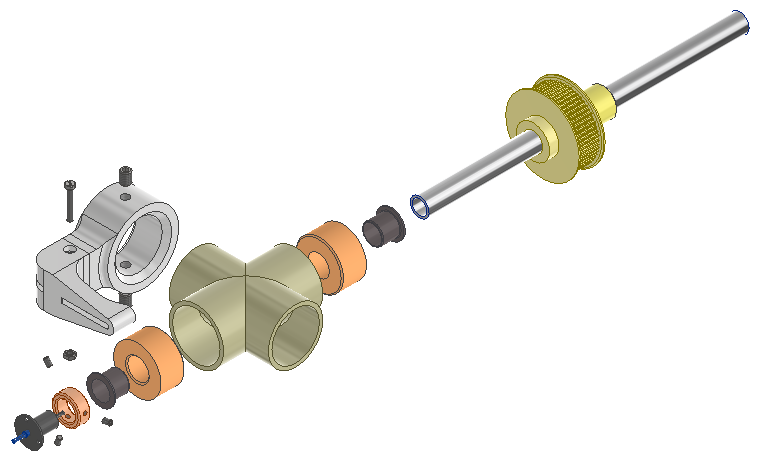
\includegraphics[width=\textwidth]{2_diss}
		\caption{Czwórnik ramy klinostatu.} 
		
		\label{fig:czwórnik}
	\end{subfigure}\vspace{15mm}%
	
	\begin{subfigure}{.8\textwidth}
		\centering
		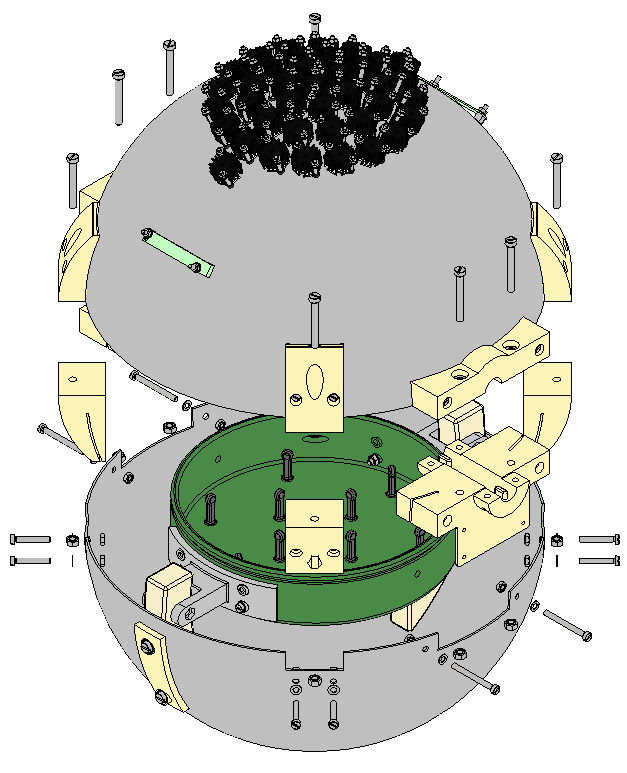
\includegraphics[scale=0.3]{Komora_tweaked_colors_exploded}
		\caption{Komora środowiskowa.} 
		\label{fig:komora}
	\end{subfigure}
	
	\caption{Przykładowe części modelu komputerowego projektu. Źródło: [opracowanie własne].}
	
\end{figure}


\section{Modyfikacje projektu}

Z uwagi na dużą złożoność realizowanego projektu, zakończył się on na etapie ukończonego modelu komputerowego. Konstrukcję całego urządzenia rozpoczęto rok po
   zakończeniu się projektu PBL w zespole dwuosobowym, w którego skład wchodziłem. Podczas
    konstrukcji napotkano wiele problemów, które nie zostały przewidziane na etapie prac
     projektowych i wymagały stworzenia nowych elementów urządzenia, bądź zmodyfikowania już
      istniejących komponentów. Oprócz tego wymagane było również stworzenie metod
       konstrukcyjnych tak, aby zachować jego kluczowe cechy oraz, aby mogło ono zostać wykonane
        bez użycia kosztownych metod obróbki takich jak wspomagana numerycznie obróbka maszynowa
         (ang. \angver{Computerized Numerical Control}, CNC). Takich poprawek stworzono bardzo
          wiele \linebreak na drodze konstrukcji urządzenia, natomiast w tym podrozdziale zostaną opisane
           dwie najbardziej kluczowe dla jego poprawnego działania.
           

\subsection{Przeciwwaga ramy klinostatu}

Podczas pierwszych prób uruchomieniowych klinostatu napotkano okresowo pojawiający się moment
 siły, który hamował ruch obrotowy urządzenia przez zbyt duże obciążenie układu napędowego. Za
  jedno ze źródeł tego problemu zidentyfikowano asymetrię obciążenia ramy klinostatu, powodowaną
   układem zmiany kierunku pasa układu napędowego komory środowiskowej, który ulokowany jest na
    rogu ramy. W tym celu na przeciwległym rogu zamontowano przeciwwagę, które generowała moment
     siły o tym samym kierunku, natomiast o przeciwnym zwrocie. Przeciwwaga składa się z
      drukowanego uchwytu oraz kawałka rury PP, która wypełniona jest piaskiem w celu
       zapewnienia odpowiedniej masy. Skonstruowana oraz zamontowana przeciwwaga przedstawiona
        została na Rys. \ref{fig:przeciwwaga}.

\begin{figure}[H]
	\centering
	\setlength{\fboxsep}{0pt}
	\setlength{\fboxrule}{1pt}
	\fbox{\includegraphics[scale=0.045]{przeciwwaga}}
	\caption{Zamontowana przeciwwaga. Źródło: [opracowanie własne].} 
	\label{fig:przeciwwaga}
\end{figure}

\subsection{Przekładnie walcowe}

Drugą bardzo istotną dla działania klinostatu modfikacją, był projekt i konstrukcja dwóch
 przekładni walcowych, które zwiększają dostępny moment obrotowy układu napędowego. Z uwagi na
  to iż klinostat przeznaczony będzie przedewszystkim do badań nad organizmami roślinnymi, jego
   prędkość obrotowa powinna mieścić się w zakresie od 1 do 2 RPM. W pierwotnej konfiguracji
    klinostat był \linebreak w stanie osiągnąć znacznie większe prędkości obrotowe, co umożliwiło
     zastosowanie wspomnianych przekładni. Zaprojektowanie przekładnie stosują redukcję obrotów
      silników 4:1. Pozwala to osiągnąć czterokrotnie wyższy moment obrotowy przed głównym kołem
       napędowym klinostatu. Model przekładni widoczny jest na Rys. \ref{fig:projekt
       	 przekładni}. Przekładnia składa się z dwóch kół zębatych o liczbie zębów odpowiednio 12 i 48. Duże koło zębate jest
          łożyskowane w dwóch miejscach przez konwencjonalne łożyska kulowe, ze względu na to iż przekładnie znajdują się w wystarczająco dużej odległości od objętości jednorodnego
            pola magnetycznego. Na małym kole zębatym umieszczono dodatkowo wpusty umożliwiajace
             montaż enkoderów, jeśli zajdzie taka potrzeba. Całość zamknięta została w korpusie
              odpowiedzialnym \linebreak za ochronę kół przez pyłem oraz zapobiegającym wydostaniu się
               smaru na zewnątrz. Skonstruowana przekładnia z nałożonym kołem pasowym
                przedstawiona jest na Rys. \ref{fig:gotowa przekładnia}. Zastosowanie przekładni
                 znacznie poprawiło działanie klinostatu, przy jednoczesnym zachowaniu wymaganej
                  prędkości obrotowej urządzenia.       


\begin{figure}
	\centering
	
	\begin{subfigure}[h]{.49\textwidth}
		\centering
		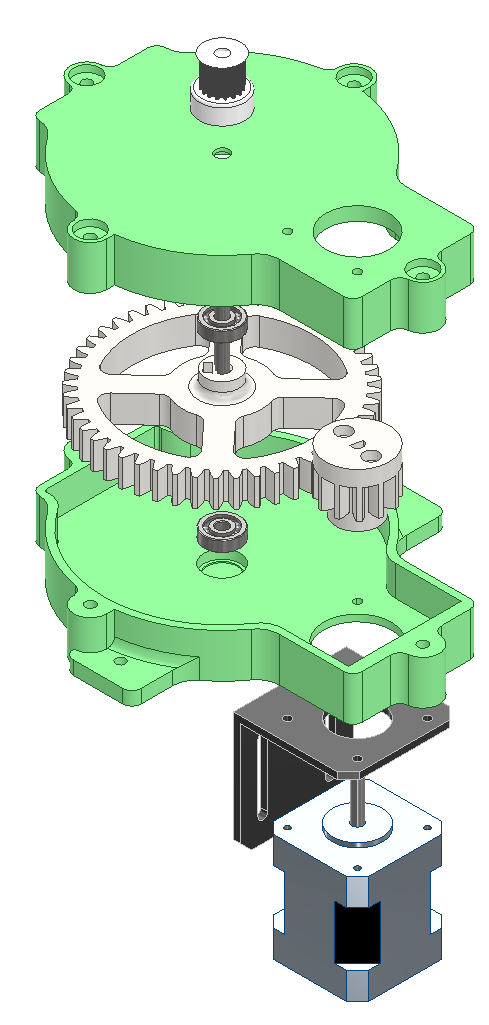
\includegraphics[width=.4\textwidth]{przekladnia_projekt_exploded_shaded}
		\caption{Projekt przekładni.} 
		\label{fig:projekt przekładni}
	\end{subfigure}
	\hfill%
	\begin{subfigure}[h]{.49\textwidth}
		\centering
		\setlength{\fboxsep}{0pt}
		\setlength{\fboxrule}{1pt}
		\fbox{\includegraphics[width=.8\textwidth, angle=-90]{przekladnia_gotowa}}
		\caption{Skonstruowana przekładnia.} 
		\label{fig:gotowa przekładnia}
	\end{subfigure}

	\caption{Przekładnie klinostatu. Źródło: [opracowanie własne].}
	
\end{figure}

\section{Komora środowiskowa}

Wewnętrzny stopień swobody klinostatu składa się z kulistej komory środowiskowej. Jej celem jest zapewnienie odpowiedniego podłoża do wzrostu badanej struktury oraz dopilnowanie optymalnych warunków wzrostowych poprzez dostarczanie wody ze składnikami odżywczymi oraz odpowiednie oświetlenie. Konieczne jest odizolowanie obiektu eksperymentu od zewnętrznych źródeł światła, aby zapewnić kontrolowane oraz powtarzalne warunki przeprowadzania eksperymentu. Komora wykonana została z globusa o średnicy \SI{320}{mm} poddanego specjalnej obróbce mechanicznej. Półsfery zostały odseparowane wzdłuż zgrzewu przy pomocy tokarki, a następnie każda z nich została poddana odpowiedniej obróbce. Model półsfer komory przedstawiono na Rys. \ref{fig:globus}. Na zawętrznej części komory wyznaczono miejsca przeznaczone do montażu kamer oraz oświetlenia. Półsfery łączone są za pomocą specjalnych, drukowanych łączników, które nasuwają się na przygotowane wcięcia i łączone są przez połączenia śrubowe (Rys. \ref{fig:łącznik_globus}). Analogicznie rozwiązanie zostało połączenie komory z wałem obrotowym. W środku komory zamontowany jest kosz uprawny, którego wysokość może być regulowana w zależności od spodziewanej wysokości struktury wzrostowej. W koszu zamontowane są specjalne elementy mocowania przewodu doprowadzającego wodę, które również wyznaczają jego spiralny tor. Wewnątrz komory rozmieszczony jest szereg czujników monitorujących warunki wzrostowe oraz jej orientację względem wektora grawitacji w czasie. Na komorze zamontowany jest również komputer niskiej mocy, odpowiedzialny za zbieranie danych z czujników i przesyłanie ich do głównej jednostki kontroli poprzez sygnał bezprzewodowy.

\begin{figure}
	\centering
	
	\begin{subfigure}[b]{.49\textwidth}
			\centering
			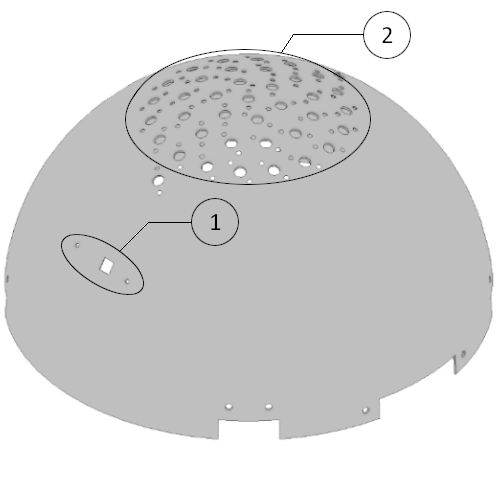
\includegraphics[width=.6\textwidth]{top_half_marked}
			\caption{Półsfera górna.} 
			\label{fig:globus_top}
	\end{subfigure}
	\hfill%
	\begin{subfigure}[b]{.49\textwidth}
			\centering
			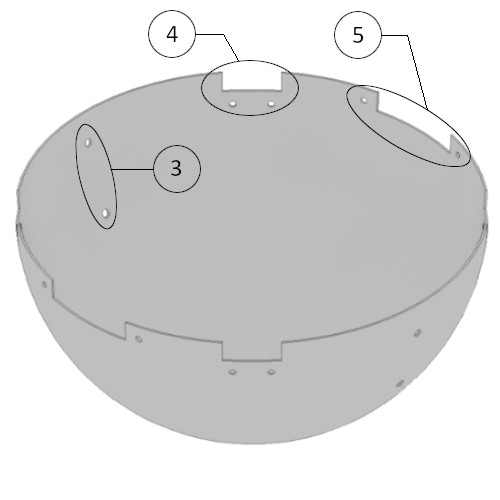
\includegraphics[width=.6\textwidth]{bot_half_marked}
			\caption{Półsfera dolna.} 
			\label{fig:globus_bot}
	\end{subfigure}
	\caption{Spreparowane półsfery z oznaczonymi elementami. \textbf{1} - otwory montażu kamery, \textbf{2} - otwory montażu oświetlenia, \textbf{3} - otwory montażu koszyka, \textbf{4} - wcięcia oraz otwory montażu łącznika półsfer, \textbf{5} - wcięcia oraz otwory montażu półsfery z wałem obrotowym. Źródło: [opracowanie własne].}
	\label{fig:globus}

\end{figure}

\begin{figure}
	
	\centering
	\includegraphics[scale=.25]{bottom_half_connector_framed}
	\caption{Łącznik montowany na półsferze komory. Źródło: [opracowanie własne].} 
	\label{fig:łącznik_globus}
	
\end{figure}

\section{Kontrola klinostatu}

Jak wspomniano w podrozdziale \ref{konstrukcja}, oba stopnie swobody klinostatu mają swoją niezależną jednostkę napędową. Jako źródło ruchu obrotowego wybrano silniki krokowe w standardzie NEMA 17, model 42BYGHM809. Są to silniki o rozdzielczości ruchu 400 kroków na pełen obrót oraz momencie obrotowym wynoszącym \SI{0,48}{Nm}. Podłączone są one do opisanych wcześniej przekładni walcowych, których wyjścia zakończone są kołami pasowymi. Ruch obrotowy jest następnie przenoszony przez pasy zębate, które ostatecznie łączą się z głównymi kołami napędowymi klinostatu na szczycie konstrukcji jego podstawy. Na silniki krokowe zdecydowano się ze względu na prostotę ich sterowania oraz możliwość dokładnego pozycjonowania w razie potrzeby rozszerzenia urządzenia o taką funkcjonalność. Silniki podłączone są bezpośrednio do obudowy zawierającej elektronikę sterującą klinostatem. Elektronika sterująca składa się z platformy Arduino Leonardo stanowiącej sterownik układu, nakładki RAMPS dla platform Arduino, dwóch sterowników silników krokowych A4988, konwertera UART/USB w celu komunikacji \linebreak z komputerem przez interfejs USB oraz przetwornicy step-up, konwertującej napięcie zasilacza 12V do 36V dla zasilania silników. W obudowie zamontowany został również wentylator chłodzący sterowniki silników. Zmontowany układ przedstawiony został na Rys. \ref{fig:elektronika}. 

\begin{figure}[ht]
	\centering
	\setlength{\fboxsep}{0pt}
	\setlength{\fboxrule}{1pt}
	\fbox{\includegraphics[width=.6\textwidth]{elektronika}}
	\caption{Elektronika klinostatu. Źródło: [opracowanie własne].} 
	\label{fig:elektronika}
\end{figure}

\graphicspath{{./Sterownik/images}}

\chapter{Sterownik kontrolera klinostatu}

Jako kontroler klinostatu rozumie się jednostkę odpowiadającą za bezpośrednie sterowanie silnikami oraz pompą wody. Jest to część systemu z którą operator urządzenia nie wchodzi bezpośrednio w interakcję, a sterowana jest ona pośrednio przez interfejs użytkownika aplikacji, poprzez system wbudowanych komend. Kontroler stanowi całkowicie odrębne urządzenie niż komputer z którego sterowany jest klinostat, natomiast nie jest ono w stanie działać samodzielnie bez kontaktu \linebreak z rdzeniem systemu. Sterownik wymagał implementacji w niskopoziomowym języku programowania, ze względu na wybór platformy z mikroprocesorem typu AVR - wybrany został w tym celu język C++.
\section{Założenia funkcjonalne sterownika}

Poniżej wymieniono funkcjonalności oraz założenia jakie musiał spełniać sterownik kontrolera klinostatu:

\begin{itemize}
	
	\item Sterowanie silników powinno być całkowicie niezależne od reszty funkcjonalności programu. Oznacza to iż odbieranie oraz wysyłanie danych przez port szeregowy powinno odbywać się równolegle z operacjami obsługującymi układ napędowy.
	\item Silniki domyślnie powinny uruchamiać się oraz zatrzymywać ze stałym przyspieszeniem tzn. prędkości obrotowe powinny zmieniać się liniowo podczas rozruchu oraz zatrzymania klinostatu.
	\item Sterownik powinien również niezależnie śledzić czas, który upłynął od rozpoczecia programu. Z pomocą odmierzania czasu obliczana jest objętość wody wpompowanej do komory środowiskowej.

\end{itemize}


\section{Platforma}

Wspomniano wcześniej iż w skład elektroniki klinostatu wchodzi płytka rozwojowa Arduino Leonardo. Jednostka mikrokontrolera (ang. \angver{microcontroller unit}, MCU) znajdująca się na tym rodzaju płytki to ATmega32U4 produkowana przez firmę Atmel. Jest to 8-bitowy MCU typu AVR, który w przypadku płytki Arduino taktowany jest za pomocą zewnętrznego oscylatora kwarcowego o częstotliwości \SI{16}{MHz} \cite{bib:nota_katalogowa}. Platforma ta została wybrana na etapie projektowym, kierując się jej dostępnością, popularnością, ceną oraz parametrami. Platformy Arduino w odniesieniu do samodzielnych kontrolerów AVR oferują znacznie prostsze metody programowania poprzez udostępnienie wielu bibliotek, które interfejsują z samymi rejestrami mikrokontrolera. Powoduje to efektywnie programowanie wyższego poziomu. Minusem takiego podejścia jest konieczność umieszczania ów bibliotek \linebreak w pamięci kontrolera, która jest ograniczona. Dodatkowo platformy arduino posiadają stały fragment kodu, który nie jest modyfikowalny przez użytkownika, tzw. bootloader, który również zajmuje część dostępnej pamięci. MCU zdecydowano się programować w czystym języku C++, z uwagi na to iż biblioteki Arduino nie oferowały wymaganej funkcjonalności. Bootloader umieszczony na platformach Arduino umożliwia programowanie przez interfejs USB. W przypadku sterownika klinostatu, bootloader usunięto, a układ programowano poprzez programator USBASP (ang. \angver{USB AVR Serial Programmer}).

\section{Rejestry mikrokontrolera}

W przypadku mikrokontrolerów AVR, kontrolowanie oraz konfiguracja ich peryferiów odbywa się poprzez konfigurowanie wewnętrznych rejestrów. Rejestry mikrokontrolera są po prostu lokalizacjami w pamięci, których wartość można odczytać lub ją zmodyfikować. Część rejestrów MCU wyznacza jego pamięć RAM (ang. \angver{Random Access Memory}), w której przechowywane są tymczasowo wartości zmiennych lub stałych, które potrzebne są w momencie wykonywania programu. Inna część rejestrów to tzw. rejestry specjalne (ang. \angver{Special Function Register}, SFR), których zadaniem jest wcześniej wspomniana kontrola oraz konfiguracja elementów mikrokontrolera.

\section{Rejestry układu czasowo-licznikowego}

Jednym z ważnych dla działania klinostatu typów SFR są rejestry odpowiedzialne za konfigurację oraz kontrolę układów czasowo-licznikowych. Układy \linebreak te cyklicznie inkrementują wartość przechowywaną w pewnych rejestrze wraz \linebreak z cyklami zegara MCU. Znając jego częstotliwość taktowania pozwala to efektywnie odmierzać czas programu. Atmega32U4 posiada 4 rejestry tego typu \cite{bib:nota_katalogowa}: 
\begin{itemize}
	\item jeden rejestr 8-bitowy, Timer/Counter 0
	\item dwa rejestry 16-bitowe, Timer/Counter 1 i 3
	\item jeden rejestr 10-bitowy o dużej szybkości, Timer/Counter 4
\end{itemize}

W sterowniku wykorzystane zostały 3 z dostępnych rejestrów układów czasowo-licznikowych. Dwa rejestry 16-bitowe przeznaczone zostały do wyznaczania interwałów czasowych między kolejnymi krokami silników, natomiast rejestr 8-bitowy przeznaczony został na odmierzanie czasu programu. Układy czasowo-licznikowe nie muszą inkrementować wartości w rejestrze co każdy cykl procesora, mogą \linebreak to robić co określoną ilość cykli. Taką ilość cykli wyznacza prescaler, który również jest konfigurowany przez odpowiednie rejestry. Wybranym trybem pracy układów czasowo-licznikowych jest tryb CTC (ang. \angver{Clear Timer on Compare Match}), który zeruje rejestr wartości układu licznika kiedy osiąga on ustaloną programowo wartość. Pozwala to na sterowanie długością interwałów pomiędzy impulsami za pomocą operacji na wartościach w  rejestrach OCRnA lub OCRnB (ang. \angver{Output Compare Register}), gdzie $n$ jest numerem układu. Konfiguracja owych układów zostanie opisana w dalszych podrozdziałach.

\section{Przerwania programowe}

Przerwania programowe są kolejną, kluczową funkcją mikrokontrolera dla spełnienia założeń sterownika klinostatu. Przerwania programowe umożliwiają przerwanie wykonywania programu w dowolnym jego miejscu i tymczasowe przekazanie kontroli do specjalnej części kodu zwanej procedurą obsługi przerwania (ang. \angver{Interrupt Service Routine}, ISR). Umożliwia to wykonywanie kluczowych operacji niezależnie od tego co w danej chwili wykonuje główny program kontrolera. Ważne jest, aby zakończyć operacje związane z ISR we względnie krótkim czasie, aby uniknąć wyzwolenia kolejnego przerwania w trakcie obsługi obecnego. Może się również zdarzyć iż obsługa przerwań zostaje wyłączona na czas wykonania ISR, co może sprawić iż zostanie ominięte zdarzenie kluczowe dla kontroli systemu. Przerwania mogą zostać wywołane przez wiele sygnałów począwszy od flag dokonania konwersji przez wewnętrzny przetwornik analogowo-cyfrowy, po wysoki stan napięciowy przyłożony do jednego z wyprowadzeń mikrokontrolera. W przypadku sterownika klinostatu przerwania wywoływane są poprzez osiągnięcie wartości zadanych \linebreak w OCRnA przez rejestry TCNTn (ilość zliczeń licznika), a procedury obsługi przerwań odpowiedzialne są za wykonanie pojedynczego kroku silnika krokowego oraz za inkrementowanie liczby milisekund upłyniętych od momentu uruchomienia programu.

\section{Sterowanie silnikami krokowymi}

Jak wspomniano w założeniach programu, wymogiem była możliwość liniowej zmiany prędkości obrotowej silników krokowych. Pomaga to odciążyć silniki podczas fazy rozruchowej klinostatu, eliminując gubione kroki. Szybkość obrotów silników krokowych zależy od częstotliwości wykonywanych kroków. Częstotliwość kroków zależna jest od czasu mijającego pomiędzy kolejnymi krokami. To właśnie ten interwał jest wielkością, która jest bezpośrednio sterowana z poziomu programu kontrolera. Zgodnie z \cite{bib:krokowe_przyspieszenie} liniowy profil prędkości można uzyskać za pomocą zależności \ref{eq:przyspieszenie}, wyznaczającej interwały pomiędzy krokami $c_n$ w kolejnych iteracjach.

\begin{equation}\label{eq:przyspieszenie}
	c_n = c_0 \big(\sqrt{n+1} - \sqrt{n} \big)
\end{equation}
gdzie $c_0$ - początkowy interwał czasowy, $n$ - numer iteracji. W taki sposób zrealizowane zostało dobieranie interwału czasowego w programie. Po osiągnięciu zadanej wartości, odpowiadającej docelowej prędkości ruchu obrotowego, interwał czasowy pozostaje stały.


\section{Komunikacja USB}

Sterowanie klinostatem odbywa się poprzez wysyłanie odpowiednich komend przez interfejs USB do kontrolera. Elementem pośrednim pomiędzy sterującym komputerem, a kontrolerem jest konwerter sygnałów protokołu USB na sygnały logiczne TTL (ang. \angver{transistor-transistor logic}) wykorzystywane przez wewnętrzny układ UART mikrokontrolera. UART również kontrolowany jest poprzez konfigurację odpowiednich SFR, a następnie odebrane dane są pobieranie z rejestru UDR1.
\begin{lstlisting}[language=C++, caption=Plik \textbf{commands.hpp}.]
// Functional commands	
#define RUN_COMMAND 0x01
#define HOME_COMMAND 0x02
#define ABORT_COMMAND 0x03
#define PAUSE_COMMAND 0x04
#define RESUME_COMMAND 0x05
#define ECHO_COMMAND 0x06
#define CONNECT_COMMAND 0x07
#define DISCONNECT_COMMAND 0x08
#define BEGIN_WATERING_COMMAND 0x09

// Notifiers
#define CLINOSTAT_CONNECTED 0x01
#define TOP_SPEED_REACHED 0x02
#define STEPPERS_STARTING 0x03
#define STOPPING_STEPPERS 0x04
#define STEPPERS_STOPPED 0x05
#define WATERING_STARTED 0x09
#define STILL_WATERING 0x0A

// Status report commands.
#define RUNNING_MODE_REPORT 0x06
#define STOPPING_MODE_REPORT 0x07
#define IDLE_MODE_REPORT 0x08
\end{lstlisting}
Powyżej widoczny jest zestaw komend, które klinostat zwraca podczas operacji oraz, które mogą zostać przez niego odebrane i zinterpretowane. Komendy znajdują się w pliku \textbf{commands.hpp} i zdefiniowane są jako dyrektywy preprocesora. Część komend wymaga odebrania 4 lub 8 kolejnych bajtów z rejestru UDR1, następujących bezpośrednio po komendzie, kolejna część wymaga odpowiedzi ze strony kontrolera klinostatu.

\section{Konfiguracja sterownika}

Konfiguracja sterownika zawarta jest w plikach \textbf{driver\_config.cpp} oraz \textbf{driver\_config.hpp}. W tych plikach znajdują się definicje oraz implementacje funkcji i makr odpowiedzialnych za odpowiednie ustawienie rejestrów związanych z układami czasowo-licznikowymi oraz aktywacją przerwań z nimi związanych. Oprócz tego w plikach tych zawarto również definicję procedury obsługi przerwania odpowiedzialnej za odmierzanie czasu.

\begin{lstlisting}[language=C++, caption=Przykładowa konfiguracja pierwszego układu czasowo-licznikowego.]
void SETUP_TIMER1_INTERRUPTS(){
	cli(); // Temporarily disable interrupts.
	TCCR1A = 0;
	TCCR1B = 0;
	TCCR1B |= (1 << WGM12); // Timer CTC mode, OCR1A as TOP.
	TCCR1B |= (1 << CS10); // Setting clock prescaler.
	TCCR1B |= (1 << CS11);
	TCNT1 = 0;
	OCR1A = STOP_INTERVAL_CHAMBER;
	sei(); // Reenable interrupts.
}
\end{lstlisting}
Układu czasowo-licznikowe 1 i 3 skonfigurowane są identycznie, pracują w trybie CTC, a ich prescaler ustawiony jest na 64 poprzez ustawienie bitów CSn0 oraz CSn1 na wartość 1 w rejestrze TCCRnB, gdzie $n$ jest numerem układu.  Jak wspomniano wcześniej zerowy układ czasowo-licznikowy przeznaczony jest do odmierzania czasu programu. W tym celu układ ten również skonfigurowany jest do pracy w trybie CTC oraz jego prescaler ustawiony jest na 64. Przy częstotliwości taktowania \SI{16}{MHz} daje to 250 tysięcy zliczeń układu w ciągu sekundy, co jest równe 250-ciu zliczeniom w ciągu jednej milisekundy. W rejestrze OCR0A zapisana została więc wartość 249, co powoduje wyzwolenie ISR co każdą milisekundę pracy programu. Liczba milisekund przechowywana jest w zmiennej typu całkowitego, bezznakowego, o wielkości 64 bitów (uint64\_t), co pozwala na śledzenie czasu programu przez $\approx5.8\cdot 10^8$ lat, znacznie przewyższając przewidywaną żywotność urządzenia.

W pliku \textbf{driver\_config.hpp} znajdują się również deklaracje wejść i wyjść mikrokontrolera. Przypisują one funkcje wykonywania kroków, włączania i wyłączania pompy oraz hamulca silników do odpowiednich wyprowadzeń mikrokontrolera. Przy zmianach fizycznej konfiguracji urządzenia, przystosowanie do niej programu jest bardzo proste, dzięki przyjętemu nazewnictwu.

\begin{lstlisting}[language=C++, caption=Konfiguracja wyprowadzeń.]
#define CHAMBER_STEP 0 // PD0 for chamber step pin.
#define FRAME_STEP 1 // PD1 for frame step pin.
#define ENABLE_PIN 4 // PB4 for enable pin for both motors.
#define PUMP_PIN 6 // PD6 for driving the pump mosfet.
\end{lstlisting}

Oprócz konfiguracji programowej ważne jest również uwzględnienie fizyczej budowy klinostatu oraz rozdzielczości silników, aby odpowiednio przeliczać prędkość ruchu obrotowego jego stopni swobody, na prędkość obrotów jego napędu. Całość mechaniki klinostatu zawarta została w pliku \textbf{clinostat\_mechanics.hpp}. Poszczególne elementy transferu ruchu obrotowego zaznaczone zostały na Rys. \ref{fig:klinostat_mechanika}.

\begin{lstlisting}[language=C++, caption=Plik \textbf{clinostat\_mechanics.hpp}.]
// Reduction of the gearbox mounted underneath the clinostat.
#define GEARBOX_REDUCTION 4 

// Number of teeth on the wheels mounted on gearboxes output.
#define STEPPER_BELT_WHEEL_TEETH 28 

// Number of teeth on the main wheels driving the clinostat.
#define MAIN_DRIVE_WHEEL_TEETH 86 

// Number of steps per revolution for the stepper motor.
#define STEPPER_STEPS_PER_REVOLUTION 400 

// Chosen mode of microstepping.
#define MICROSTEP_DIVISION 16 

// Number of steps per revolution considering the microstepping.
#define STEPS_PER_REVOLUTION (STEPPER_STEPS_PER_REVOLUTION*MICROSTEP_DIVISION)
\end{lstlisting}

\begin{figure}[h]
	
	\centering
	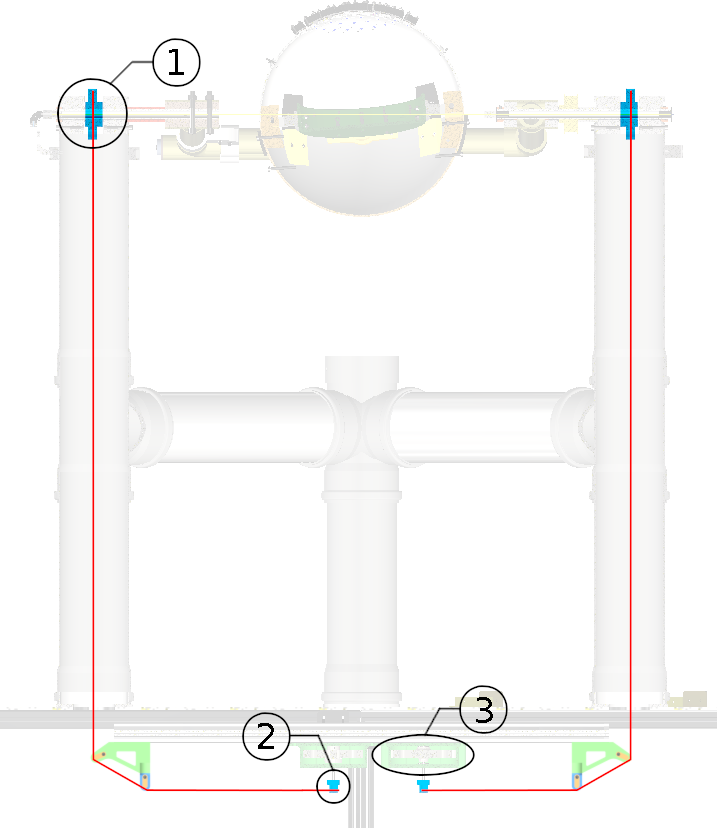
\includegraphics[scale=0.3]{klinostat_przekroj}
	\caption{Elementy mechaniki klinostatu, widok przekroju. Czerwoną linią zaznaczona jest ścieżka transferu ruchu obrotowego przez pasy. \textbf{1} - główne koło napędowe klinostatu, \textbf{2} - koło pasowe przekładni, \textbf{3} - przekładnia o redukcji 4:1 do której przymocowany jest silnik krokowy. Źródło: [opracowanie własne].} 
	\label{fig:klinostat_mechanika}
\end{figure}

Zależność \ref{eq:obroty_klinostat} przedstawia sposób w jaki wyznaczany jest minimalny interwał czasowy układów czasowo-licznikowych na podstawie prędkości zadanej przez operatora.

\begin{equation}\label{eq:obroty_klinostat}
	c_{min} = \frac{f_{CPU} \cdot 60 \cdot N_S}{P_{DIV} \cdot R_{MOT} \cdot \omega_T \cdot R_G \cdot N_M}
	\vspace{3mm}
\end{equation}
gdzie $f_{CPU}$ - częstotliwość taktowania MCU  [Hz], $N_S$ - liczba zębów na kole pasowym przekładni, $P_{DIV}$ - wartość prescalera układu czasowo-licznikowego, $R_{MOT}$ - rozdzielczość silników krokowych [kroki/obrót], $\omega_T$ - docelowa prędkość obrotów danego stopnia swobody klinostatu [RPM], $R_G$ - redukcja obrotów przekładni (4 w przypadku redukcji 4:1), $N_M$ - liczba zębów na głównym kole napędowym klinostatu. Jednostką wyznaczanego wyniku jest liczba zliczeń układu czasowo-licznikowego.

\section{Schemat blokowy sterownika klinostatu}

Na Rys. \ref{fig:schemat_sterownik} przestawiony został przebieg programu kontrolera klinostatu\linebreak w postaci schematu blokowego. Po podłączeniu zasilania logiki klinostatu program od razu rozpoczyna działanie od inicjalizacji używanych układów oraz wyprowadzeń MCU. Następie kontrola przekazywana jest do pętli głównej, która będzie wykonywać się cyklicznie, aż do odłączenia zasilania układu. Pętla główna składa się z funkcji sprawdzającej czy w buforze portu szeregowego znajduje się komenda czekająca na odebranie i interpretację. Jeśli taka komenda została znaleziona,\linebreak to wywoływana jest funkcja \textbf{handleSerial}, której zadaniem jest odebranie ów komendy i w zależności od jej rodzaju odebrać lub nie, dodatkowe dane po niej następujące. Jeśli odebrana komenda wpływa na zmianę trybu pracy urządzenia, to aktualizowana jest flaga obecnego statusu programu. W dalszym ciągu sterownika obsługiwane jest działanie pompy - sprawdzane jest czy obecnie pompa jest włączona, jeśli jest to sprawdzany jest czas, który upłynął od jej włączenia.\linebreak W zależności ile taki czas wynosi pompa jest wyłączana, lub pozostaje włączona. Na końcu pętli wykonywna jest funkcja \textbf{checkMotorStatus}, która sprawdza flagi określające status silników, wyłączając działanie procedur obsługi przerwań w razie takiej konieczności (powoduje to zatrzymanie silników). Podczas działania głównej pętli aktywne są również trzy procedury obsługi przerwań, które niezależnie od jej statusu, sterują silnikami krokowymi oraz odmierzają czas.
\begin{figure}[H]
	\centering
	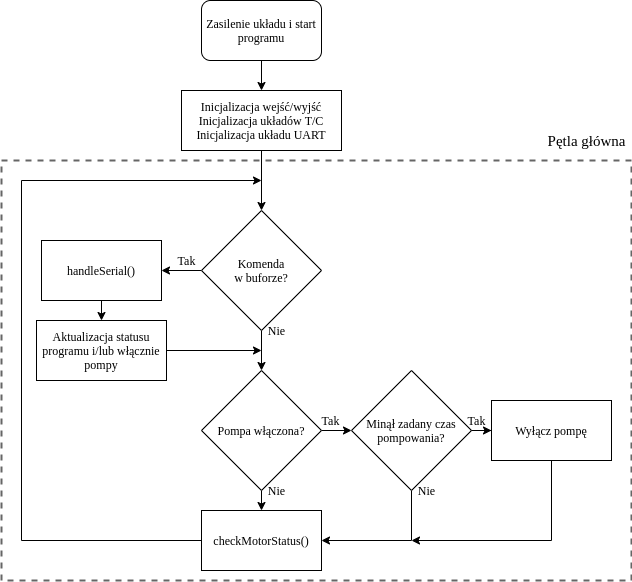
\includegraphics[scale=0.5]{sterownik_schemat}
	\caption{Schemat blokowy programu kontrolera. Źródło: [opracowanie własne].} 
	\label{fig:schemat_sterownik}
\end{figure}


\section{Kompilacja i programowanie}

Z uwagi na małą złożoność struktury plików sterownika nie zdecydowano się\linebreak na użycie narzędzi budowy projektów takich jak CMake. W ramach ułatwienia procesu kompilacji oraz programowania układu, napisano prosty plik reguł Makefile. W pliku tym zawarto trzy reguły:
\begin{itemize}
	\item all: reguła odpowiedzialna za kompilację kodu źródłowego do pliku binarnego .hex
	\item install: reguła odpowiedzialna za zaprogramowanie układu z użyciem pliku .hex i programatora USBASP
	\item clean: metoda usuwająca pliki pośredniczące w procesie kompilacji
\end{itemize}
Taki zestaw reguł okazał się całkowicie wystarczający w procesie rozwoju programu oraz pozwala nawet osobie bez specjalnej wiedzy na samodzielne zaprogramowanie układu. Projekt można skompilować oraz zaprogramować na każdym systemie z zainstalowanym łańcuchem narzędziowym (ang. \angver{toolchain}) \textbf{avr-gcc} oraz narzędziem \textbf{avrdude}.

\begin{lstlisting}[caption=Makefile sterownika.]
CC=avr-gcc
CFLAGS= -Os -DF_CPU=16000000UL -mmcu=atmega32u4

all: clinostat-stepper-driver.out
%.out: %.cpp
	$(CC) $(CFLAGS) **.cpp -o $@
%.hex: %.out
	avr-objcopy -O ihex -R .eeprom $< $@

install.%: %.hex
	avrdude -F -V -c usbasp -p m32u4 -b 115200 -U flash:w:$<

clean:
	rm -f *.out
\end{lstlisting}

\graphicspath{{./Aplikacja/images}}

\chapter{Aplikacja pulpitowa}

Aplikacja będąca obiektem tego podrozdziału stanowi rdzeń systemu kontroli, dzięki któremu operator urządzenia jest nim w stanie sterować oraz zbierać z jego pomocą dane. Zawiera ona moduły do komunikacji ze wszystkimi częściami urządzenia oraz zestaw wykresów aktualizowanych w czasie rzeczywistym. Pomimo względnie prostych funkcji, aplikacja posiada złożoną strukturę ze względu na rówoległą obsługę różnych dróg komunikacji. Struktura ta w szczegółach opisana zostanie  w dalszej części tego rozdziału.

\section{Rola i założenia aplikacji}

Aplikacja była rozwijana mając na uwadze poniższe założenia:
\begin{itemize}
	\item Powinna umożliwiać oparatorowi zadanie prędkości obu stopni swobody klinostatu oraz objętości wody, która ma zostać dostarczona co wskazany przez operatora interwał czasowy.
	\item Powinna dawać dostęp do danych o orientacji komory względem wektora grawitacji, uśrednionej grawitacji i temperatury z ostatnich 60 sekund. Dane odnośnie wilgotności podłoża z uwagi na korozję czujnika przeprowadzane\linebreak są znacznie rzadziej. Dodatkowo na jednym z wykresów przedstawiana ma być transformata Fouriera sygnału uzyskanego z akcelerometru.
	\item Powinna posiadać podstawowe zabezpieczenia, aby uniemożliwić operatorowi zawieszenie urządzenia poprzez nieświadome wykonanie operacji niedozwolonych. Powinny również znaleźć się w niej zabezpieczenia obsługujące błędy generowane przez fizyczne odłączenie klinostatu w momencie gdy program zakłada iż jest on podłączony.
	\item Powinna w tle posiadać uruchomiony moduł komunikacji bezprzewodowej\linebreak z komorą środowiskową. Połączenie to służyć ma wymianie danych oraz nastawie intensywności oświetlenia.
	\item Oprator powinien mieć możliwość zapisania zebranych wyników pomiarów do pliku .csv.
	\item Powinien istnieć podstawowy system komunikatów, który będzie informować operatora o rezultatach jego operacji.
\end{itemize}

\section{Wybrany język i biblioteki} \label{aplikacja_implementacja}

W celu implementacji aplikacji wybrany został język Python. Wybór ten motywowany był moją dobrą znajomością tego języka oraz poprzednim doświadczeniem w tworzeniu aplikacji z graficznym interfejsem użytkownika w tym języku. Interfejs został stworzony z użyciem biblioteki \textbf{Tkinter}, która oferuje względnie proste tworzenie takich aplikacji w konwencji programowania obiektowego, z której\linebreak to intensywnie korzystano podczas rozwoju programu. Do realizacji łącza bezprzewodowego z komorą środowiskową wykorzystano bibliotekę \textbf{socket}, pozwalającą na utworzenie takiego łącza w lokalnej sieci poprzez protokół TCP (ang. \angver{Transmission Control Protocl}). Do działania programu niezbędna okazała się biblioteka \textbf{threading}, pozwalająca na współbieżne wykonywanie różnych jego części. Transformacja Fouriera liczona jest 15 razy na sekundę z użyciem biblioteki \textbf{scipy},\linebreak a obliczenia te są zrównoleglone za pomocą biblioteki \textbf{multiprocessing} w celu ich przyspieszenia. Wykresy tworzone są wykorzystując popularną bibliotekę \textbf{matplotlib}. Oprócz tego wykorzystano również wiele innych modułów takich jak \textbf{pyserial}, \textbf{yaml}, \textbf{queue} czy \textbf{numpy} w różnych, mniej znaczących celach.

\section{Podział programu na wątki} \label{watki}

Cała aplikacja składa się w jednym momencie z trzech rodzajów wątków:
\begin{itemize}
	\item Wątku głównego - odpowiedzialnego za działanie całej aplikacji oraz tworzenie wykresów.
	\item Wątku serwera TCP - odpowiedzialnego za obsługę przychodzących pakietów danych przez websocket oraz wysyłanie odpowiedzi.
	\item Wątków obsługi portu szeregowego - tworzonych jedynie tymczasowo w momencie gdy należy wysłać i/lub odebrać komendę przez magistralę USB\linebreak z klinostatem.
\end{itemize}
Docelowo wątek główny miał być odpowiedzialny wyłącznie za uruchamianie innych wątków oraz działanie aplikacji, natomiast tworzenie i akutualizacja wykresów miała być rezultatem działania innego, dodatkowego wątku. Takie rozwiązanie okazało się niemożliwe, ze względu na konstrukcję biblioteki matplotlib, która uniemożliwia tworzenie wykresów przez wątki inne niż główny. Związane jest\linebreak to z tym iż biblioteka ta nie została stworzona w konwencji \angver{threadsafe} - bezpiecznej w działaniach między wątkami. Przy programowaniu wielowątkowym należy zwracać uwagę na występowanie tzw. wyścigów (ang. \angver{race condition}), które występują w momencie gdy przynajmniej dwa, różne wątki próbują uzyskać dostęp\linebreak do tej samej, dzielonej zmiennej. Występowanie takich wyścigów jest znane w bibliotece matplotlib, a więc wykorzystywana może być ona wyłącznie w obrębie wątku głównego. Rozwiązaniem problemu wyścigów jest wykorzystanie różnego rodzaju struktur synchronizacyjnych takich jak semafory czy zamki, które zapobiegają ich występowaniu. Z tego rodzaju struktur korzysta również aplikacja.\\

Wątek serwera TCP jest uruchamiany przez użytkownika za pomocą odpowiedniego przycisku. Pozostaje on uruchomiony w tle aż do momentu, w którym operator postanowi zakończyć komunikację. Jego rolą jest odbieranie danych pomiarowych wysłanych z komputera komory środowiskowej oraz odesłanie odpowiedzi zawierającej informacje o obecnie ustawionym poziomie oświetlenia. Ze względu na to iż dane te muszą zostać przekazane do wątku głównego, wymiana ta zachodzi poprzez wykorzystanie struktur \textbf{Queue} z biblioteki \textbf{queue}, które zapobiegają wyścigom pomiędzy wątkami.\\

Ostatnim z wątków występujących w programie jest wątek odpowiedzialny\linebreak za obsługę portu szeregowego, realizującego komunikację z kontrolerem klinostatu. Jego zadaniem jest uzyskanie dostępu do wcześniej utworzonego połączenia szeregowego, wysłanie pożądanej komendy, a następnie uzyskanie odpowiedzi ze strony klinostatu. Takich wątków w jednej chwili może istnieć kilka, ponieważ\linebreak w programie zachodzą również zautomatyzowane procesy, które wysyłają komendy\linebreak do klinostatu. Natomiast dostęp do połączenia w tym samym czasie może uzyskać wyłącznie jeden z nich ze względu na wykorzystanie struktury synchronizacyjnej \textbf{lock}. Powoduje to efektywne kolejkowanie operacji wykonywanych na porcie szeregowym. W przeciwnym wypadku program zwróciłby błąd, gdy połączenie\linebreak z klinostatem zostałoby otwarte po raz drugi. Schemat struktury wątkowej przedstawiony został na Rys. \ref{fig:watki}.

\begin{figure}
	
	\centering
	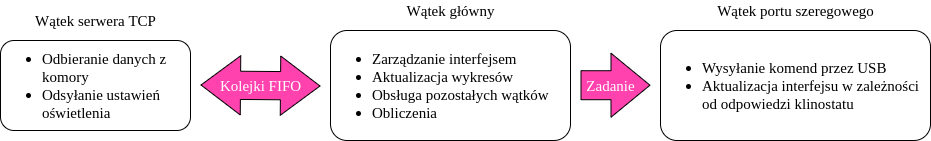
\includegraphics[scale=0.46]{schemat_watki}
	\caption{Schemat budowy wątkowej aplikacji. Źródło: [opracowanie własne].} 
	\label{fig:watki}
	
\end{figure}

\section{Graficzny interfejs użytkownika}

Ten podrozdział poświęcony został opisowemu przedstawieniu graficznego interfejsu użytkownika. Podczas jego tworzenia kierowano się tym, aby był on czytelny, intuicyjny w obsłudze oraz responsywny, aby dawać użytkownikowi pewność iż dokonywane przez niego operacje przynoszą skutek. Interfejs domyślnie po starcie programu jest w znacznej części nieaktywny. Odpowiednie jego sekcje aktywują się gdy pomyślnie zostanie nawiązana komunikacja z kontrolerem klinostatu lub komputerem komory środowiskowej. Taka zmiana uwydatniana jest za poprzez zmianę koloru części interfejsu. Nastawa prędkości klinostatu odbywa się za pomocą dwóch suwaków, które pozwalają na regulację prędkości obu stopni swobody od \SI{0,1}{RPM} do \SI{5}{RPM} z rozdzielczością \SI{0,1}{RPM}. Bezpośrednio obok suwaków znajdują się przyciski odpowiedzialne za uruchomienie bądź zatrzymanie klinostatu. Podgląd tej sekcji interfejsu widoczny jest na Rys. \ref{fig:silniki_gui}. Przyciski oraz ich funkcje, składające się na tę część interfejsu to:
\begin{itemize}
	\item \textbf{Abort} - przycisk natychmiastowo zatrzymujący klinostat bez rampy prędkości. Odpowiada również za wyłączenie hamulców silników gdy klinostat został już wcześniej zatrzymany.
	\item \textbf{Run} - przycisk odpowiedzialny za wysłanie do klinostatu komendy o rozpoczęciu ruchu oraz przekazaniu mu parametrów prędkości.
	\item \textbf{Pause} - przycisk zatrzymujący klinostat poprzez liniową zmianę prędkości. Po zatrzymaniu, hamulce silników pozostają włączone.
	\item \textbf{Resume} - wznowienie ruchu klinostatu po wcześniejszym zatrzymaniu go poprzez komendę Pause.
	\item \textbf{Echo} - przycisk wysyłający komendę do klinostatu, która wymaga odpowiedzi ze strony jego kontrolera. Jeśli kontroler zwraca jedną z przewidywanych komend, jej skutek wyświetlany jest w aplikacji. Jeśli podczas komunikacji nastąpił błąd, stan całego programu jest resetowany.
\end{itemize}

\begin{figure}
	\centering
	
	\begin{subfigure}[h]{.49\textwidth}
		\centering
			\setlength{\fboxsep}{0pt}
		\setlength{\fboxrule}{1pt}
		\fbox{\includegraphics[scale=1.5]{kontrola_silników}}
		\caption{Nieaktywny interfejs.}
		\label{fig:silniki_gui_nieaktywne}
	\end{subfigure}
	\hfill%
	\begin{subfigure}[h]{.49\textwidth}
		\centering
		\setlength{\fboxsep}{0pt}
		\setlength{\fboxrule}{1pt}
		\fbox{\includegraphics[scale=1.5]{kontrola_silników_aktywny}}
		\caption{Aktywny interfejs.} 
		\label{fig:silniki_gui_aktywne}
	\end{subfigure}
	
	\caption{Interfejs sterowania silnikami. Źródło: [opracowanie własne].}
	\label{fig:silniki_gui}
	
\end{figure}

Sterowanie nawadnianiem odbywa się w podobny sposób. Do dyspozycji\linebreak są dwa suwaki określające jak często woda ma zostać doprowadzona do środka komory środowiskowej oraz jaka jej objętość za każdym razem będzie do niej trafiać.\linebreak Na ten blok interfejsu przypadają również trzy przyciski:
\begin{itemize}
	\item \textbf{Start cycle} - rozpoczęcie planu nawadniania według ustawionych parametrów. Jeśli interwał czasowy lub objętość nawadniania zostały ustawiony\linebreak na wartość zerową, wciśnięcie tego przycisku spowoduje pojawienie się stosownego komunikatu, a cykl się nie rozpocznie.
	\item \textbf{Stop cycle} - przycisk zatrzymujący obecny cykl nawadniania i odblokowywujący ponownie jego nastawę.
	\item \textbf{Force cycle} - przycisk powodujący natychmiastowe wykonanie akcji pompowania o nastawionym parametrze objętościowym. Jeśli w czasie wciśnięcia tego przycisku proces nawadniania trwa, kontroler klinostatu wykryje taką sytuację i zwróci stosowny komunikat do aplikacji.
\end{itemize}
Część interfejsu odpowidzialna za nawadnianie widoczna jest na Rys. \ref{fig:nawadnianie_gui}.\\

\begin{figure}
	\centering
	
	\begin{subfigure}[h]{.49\textwidth}
		\centering
		\setlength{\fboxsep}{0pt}
		\setlength{\fboxrule}{1pt}
		\fbox{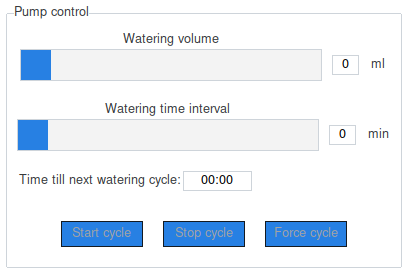
\includegraphics[scale=1.5]{pompa}}
		\caption{Nieaktywny interfejs.}
		\label{fig:woda_gui_nieaktywne}
	\end{subfigure}
	\hfill%
	\begin{subfigure}[h]{.49\textwidth}
		\centering
		\setlength{\fboxsep}{0pt}
		\setlength{\fboxrule}{1pt}
		\fbox{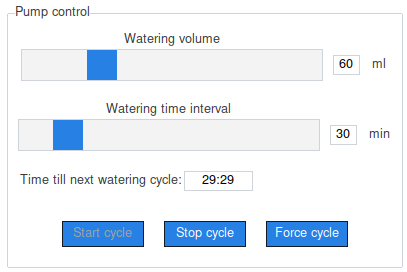
\includegraphics[scale=1.5]{pompa_cykl}}
		\caption{Trwający cykl.} 
		\label{fig:woda_gui_aktywne}
	\end{subfigure}
	
	\caption{Interfejs cyklu nawadniania. Źródło: [opracowanie własne].}
	\label{fig:nawadnianie_gui}
	
\end{figure}\
Kolejnym modułem interfejsu jest kontrola oświetlenia komory środowiskowej widoczna na Rys. \ref{fig:oswietlacz_gui}. W przeciwieństwie do wcześniej opisanych częśći, ten segment pozostaje nieaktywny aż do momentu nawiązania bezprzewodowej komunikacji z komputerem komory klinostatu. Regulacja odbywa się za pomocą określenia intensywności oświetlenia w zakresie od 0 do 100 \%. Wartość ta bezpośrednio odpowiada wypełnieniu sygnału PWM (ang. \angver{Pulse Width Modulation}), którym sterowane są odpowiednie sekcje oświetlenia. Nastawa przekazywana jest przy okazji wymiany informacji z komputerem komory środowiskowej.\\

\begin{figure}[h]
	\centering
	
	\begin{subfigure}[h]{.49\textwidth}
		\centering
		\setlength{\fboxsep}{0pt}
		\setlength{\fboxrule}{1pt}
		\fbox{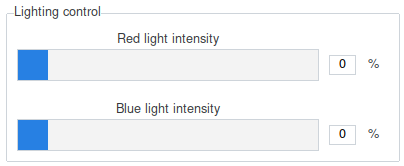
\includegraphics[scale=1.5]{oswietlacz}}
		\caption{Nieaktywny interfejs.}
		\label{fig:oswietlacz_gui_nieaktywne}
	\end{subfigure}
	\hfill%
	\begin{subfigure}[h]{.49\textwidth}
		\centering
		\setlength{\fboxsep}{0pt}
		\setlength{\fboxrule}{1pt}
		\fbox{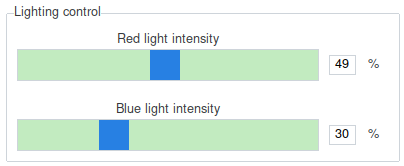
\includegraphics[scale=1.5]{oswietlacz_aktywny}}
		\caption{Aktywny interfejs.} 
		\label{fig:oswietlacz_gui_aktywne}
	\end{subfigure}
	
	\caption{Nastawa oświetlenia. Źródło: [opracowanie własne].}
	\label{fig:oswietlacz_gui}
		
\end{figure}
Jak wspomniano w podrozdziale \ref{aplikacja_implementacja}, połączenie z komputerem komory środowiskowej realizowane jest z użyniem protokołu TCP. Odbywa się to poprzez uruchomienie serwera TCP za pośrednictwem aplikacji przy użyciu przycisku \textbf{Run server}. Jeśli połączenie zostało nawiązane wyświetlony zostanie stosowny komunikat. W przypadku wystąpienia błędu, również zostanie on wyświetlony w wewnętrznej konsoli programu. Aby zerwać połączenie, należy serwer zamknąć naciskając przycisk \textbf{Close server}. Moduł odpowiedzialny za te intrukcje jest widoczny na Rys. \ref{fig:tcp_gui}.\\

\begin{figure}[h]
	
	\centering
	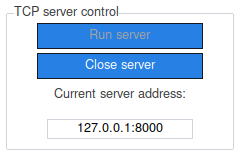
\includegraphics[scale=2]{serwer}
	\caption{Kontrola serwera TCP. Źródło: [opracowanie własne].} 
	\label{fig:tcp_gui}
	
\end{figure}

Bardzo istotnym elementem interfejsu jest konsola w której wyświetlane są komunikaty generowane przez aplikację. Została ona zintegrowana razem z kontrolą połączenia z klinostatem do jednego modułu, przedstawionego na Rys. \ref{fig:konsola_gui}.\linebreak Na ten moduł składa się rozwijane menu z dostępnymi urządzeniami podłączonymi\linebreak do portów USB komputera oraz zestaw czterech przycisków:
\begin{itemize}
	\item \textbf{Refresh ports} - przycisk aktualizujący obecnie dostępne urządzenia podłączone do portów szeregowych. Pozwala to wykryć urządzenia, które zostały podłączone do komputera po uruchomieniu aplikacji.
	\item \textbf{Connect} - przycisk inicjujący komunikację z klinostatem przez port USB. Wciśnięcie tego przycisku wysyła komendę do wybranego portu i następnie czeka na odpowiedź. Jeśli otrzymany, powrotny komunikat zgadza się ze spodziewaną komendą klinostatu, interfejs aplikacji zostaje włączony. W konsoli wyświetlany jest stosowny komunikat o błędzie lub pomyślnym połączeniu.
	\item \textbf{Disconnect} - zerwanie połączenia z klinostatem poprze wysłanie odpowiedniej komendy.
	\item \textbf{Clear logs} - przycisk czyszczący komunikaty obecnie znajdujące się w konsoli.
	
\end{itemize}

\begin{figure}[h]
	
	\centering
	\setlength{\fboxsep}{0pt}
	\setlength{\fboxrule}{1pt}
	\fbox{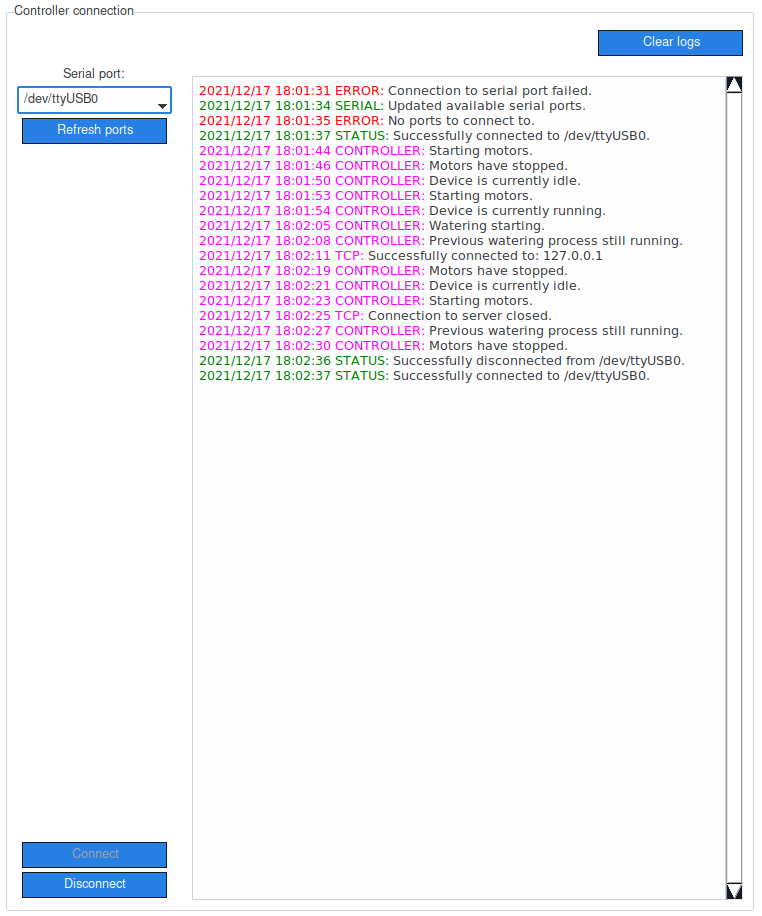
\includegraphics[scale=1.7]{konsola_serial}}
	\caption{Konsola oraz interfejs połączenia szeregowego. Źródło: [opracowanie własne].} 
	\label{fig:konsola_gui}
	
\end{figure}

Cały interfejs podzielony jest na dwie zakładki. Wszystkie dotychczas wymienione elementy znajdują się w zakładce \textit{Clinostat control}. Druga zakładka (\textit{Diagnostics}) zawiera wykresy przedstawiajace zbierane dane w czasie rzeczywistym.\linebreak Na samym dole zakładni znadjują się dwa przyciski, których zadaniem jest zapisanie lub wyczyszczenie aktualnych danych. Wciśnięcie przycisku \textbf{Save data} spowoduje pojawienie się okna dialogowego w którym należy wybrać ścieżkę oraz nazwę zapisywanego pliku csv. Przycisk \textbf{Clear data} pyta użytkownika czy\linebreak na pewno chce usunąć zebrane dane, a następnie wykonuje jego wolę. Przykładowe wykresy z rzeczywistymi danymi przedstawione zostały na Rys. \ref{fig:wykresy_gui}.

\begin{figure}[h]
	\centering
	
	\begin{subfigure}[h]{.49\textwidth}
		\centering
		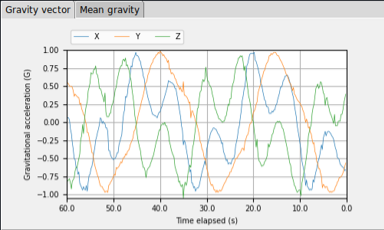
\includegraphics[scale=1.7]{grav_surowe}
		\caption{Dane z akcelerometru.}
		\label{fig:grav_raw}
	\end{subfigure}
	\hfill%
	\begin{subfigure}[h]{.49\textwidth}
		\centering
		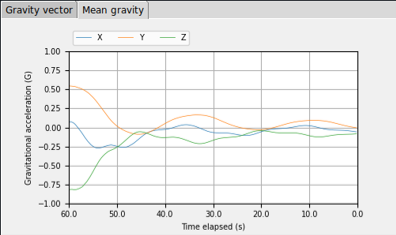
\includegraphics[scale=1.7]{grav_sr}
		\caption{Uśrednione wartości grawitacji.} 
		\label{fig:grav_mean}
	\end{subfigure}
	
	\caption{Przykładowe wykresy. Źródło: [opracowanie własne].}
	\label{fig:wykresy_gui}
	
\end{figure}

\section{Drzewo projektu}

Aplikacja napisana jest w konwencji obiektowej. Aby zachować zorganizowaną strukturę kodu źródłowego podzielony został on na wiele plików, w których znajdują się definicje klas o podobnych cechach lub działaniu. Rozdział ten służy przedstawieniu struktury aplikacji oraz krótkiemu opisowi, funkcji jakie pełni każdy\linebreak z plików. Drzewo programu widoczne jest na Rys. \ref{fig:drzewo}. Plikiem uruchomieniowym jest plik \textbf{main.py}, który zawiera definicję klasy samej aplikacji oraz klasę menedżera interfejsu, odpowiedzialnego za zmiany aktywności jego elementów. Poszczególne moduły aplikacji odnoszą się do interfejsu właśnie przez ten obiekt,\linebreak co znacznie poprawia czytelność oraz organizację kodu. W folderze \textit{config} znajduje się plik konfiguracyjny \textbf{config.yaml}, który zawiera adres oraz port na których postawiony ma zostać serwer TCP. Folder \textit{modules} zawiera kolejne katalogi \textit{backend}, \textit{gui} oraz \textit{properties}. W katalogu \textit{backend} umieszczono wszystkie pliki zawierające obiekty sterujące lub tworzące mechanizmy aplikacji, które nie są widoczne dla użytkownika. Zawierają się w tym pliki \textbf{clinostat\_com.py} zawierający moduł komunikacyjny klinostatu, \textbf{custom\_thread.py} w którym znajduje się zmodyfikowana klasa wątku oraz plik \textbf{data\_socket.py}, który zawiera definicję obiektu serwera TCP. Katalog \textit{gui} zawiera pliki związane z elementami interfejsu graficznego, na które składają się \textbf{segments.py} zawierający definicje poszczególnych modułów interfejsu oraz plik \textbf{custom\_tk\_widgets.py}, który zawiera pojedyncze, zmodyfikowane elementy interfejsu stworzone na potrzeby aplikacji. W ostatnim folderze \textit{properties} znajduje się plik \textbf{properties.py}, który zawiera specjalnie przygotowane struktury danych, przechowywujące zmienne, flagi oraz obiekty kluczowe dla działania aplikacji.

\begin{figure}[h]
	
	\centering
	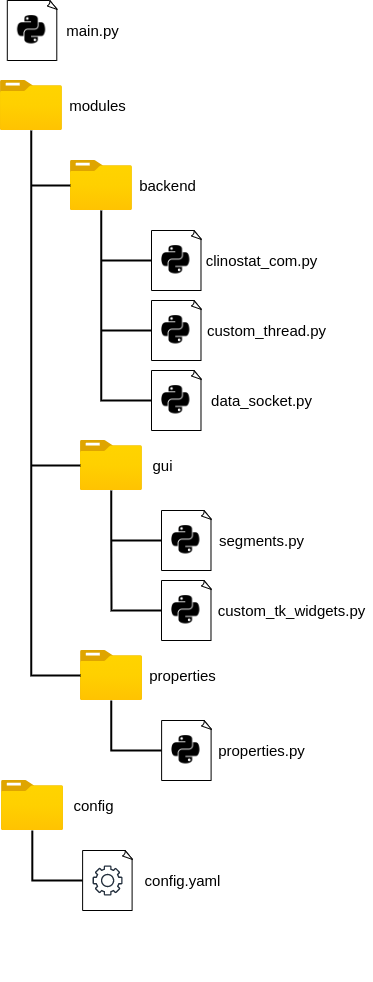
\includegraphics[scale=.34]{tree}
	\caption{Struktura plików aplikacji. Źródło: [opracowanie własne].} 
	\label{fig:drzewo}
	
\end{figure}
\section{Zabezpieczenia aplikacji}

Po wstępnym ukończeniu aplikacji poddano ją szczegółowym testom, przeprowadzanym przez kilka niezwiązanych z nią wcześniej osób. Miało to na celu wykrycie ukrytych błędów, przetestowanie jak największej ilości kombinacji wysłanych komend, zbadanie reakcji aplikacji na nadużycie dostępnych operacji oraz innych niepożądanych efektów, których wystąpienie nie zostało przewidziane na etapie jej tworzenia. Testy te pozwoliły na stworzenie zabezpieczeń uniemożliwiających operatorowi urządzenia wykonania niedozwolonych operacji oraz wykrywających konflikty powstałych na drodze interakcji operacji użytkownika oraz zachodzących\linebreak w tle zautomatyzowanych procesów. Najprostszym zabezpieczeniem obecnym\linebreak w aplikacji jest tymczasowa dezaktywacja interfejsu odpowiedzialnego za komendy wysyłane przez port szeregowy. Jeśli wysłana komenda powoduje wysłane odpowiedzi ze strony kontrolera klinostatu, to część elementów interfejsu zostaje dezaktywowana do czasu jej otrzymania, lub do maksymalnego czasu oczekiwania. Zapobiega to wysłaniu przez użytkownika komendy w momencie gdy do klinostatu przekazywane są przykładowo bajty określające prędkość obrotów. Aplikacja posiada również zautomatyzowany system wysyłania komendy nawadniania w momencie kiedy minął odpowiedni czas. Stwarza to możliwość próby wysłania takiej komendy podczas np. oczekiwania na odpowiedź ze strony klinostatu. Brak zabezpieczeń spowodowałby uzyskanie nieprawidłowej odpowiedzi z urządzenia co doprowadziłoby do błędu. Problem ten rozwiązano tworząc obiekt specjalnego wątku, który wykorzustuje strukturę synchronizacyjną \textbf{lock}, aby uniemożliwić dostęp innym wątkom do portu szeregowego podczas oczekiwania na komendę. Po zakończeniu pracy wątek odblokowywuje port szeregowy i zakolejkowana instrukcja zostaje wysłana. Klinostat może zostać również fizycznie odłączony od komputera podczas pracy. Aplikację oraz urządzenie chronią tutaj dwa mechanizmy. Pierwszy\linebreak z nich wynika z samej konstrukcji elektroniki klinostatu, która wymaga połączenia z komputerem przez port USB, aby uzyskać zasilanie sekcji logicznej. Zerwanie połączenia automatycznie spowoduje odcięcie zasilania kontrolera i zatrzymanie klinostatu. Natomiast wysłanie komendy do odłączonego portu wygeneruje błąd w aplikacji, co skutkuje jej zawieszeniem. Rozwiązaniem tego problemu było stworzenie specjalnej metody \textbf{device\_likely\_unplugged} klasy aplikacji, która wykonywana jest przez wątek obsługujący port szeregowy w momencie zgłoszenia przez niego wyjątku (ang. \angver{exception}). Wykonanie tej metody powoduje całkowite zresetowanie aplikacji i wyświetlenie stosownego komunikatu o błędzie, sugerującego sprawdzenie połączenia przewodu USB.
\begin{lstlisting}[language=Python,caption={Metoda wykrywająca odłączone urządzenie.}]
def device_likely_unplugged(self) -> None:

	try:
		self.params["device"].close_serial()
		
	except clinostat_com.ClinostatCommunicationError:
		pass
		
	self.params["device"] = None
	self.interface_manager.ui_modes_reset()
	self.flags["pumping"] = False
	self.trackers = properties.AppTrackers()
\end{lstlisting}

\graphicspath{{./Komora/images/}}

\chapter{Program komputera komory środowiskowej}

Komora środowiskowa jest częścią urządzenia, w której zachodzi wzrost badanej struktury biologicznej. Kluczowe dla jej wzrostu jest zachowanie pewnych cech takich jak odpowiednia ilość dostępnej wody w jej podłożu wzrostowym lub odpowiednie oświetlenie. Oprócz tego przydatne może okazać się śledzenie parametrów takich jak temperatura. Komora środowiskowa jest też miejscem docelowym, gdzie działanie grawitacji jest eliminowane poprzez klinorotację. Muszą się więc znajdować również w niej czujniki, które jakość symulowanej mikrograwitacji będą monitorować.

\section{Platforma}

Wybór platformy komputera komory środowiskowej został dokonany na etapie tworzenia projektu urządzenia. Wybrany został komputer Raspberry Pi Zero ze względu na niski pobór energii, co było kluczowe ze względu na ograniczenia prądowe złącz ślizgowych oraz generowane przez komputer pola magnetyczne, które w przypadku wyższych mocy mogą zaburzyć jednorodność pola. Posiada on również wbudowany moduł Wi-Fi za pomocą którego zrealizowano połączenie bezprzewodowe. Umożliwia to także zdalną obsługę komputera poprzez standard SSH (ang. \angver{Secure Shell}) w momencie gdy nastąpi awaria oprogramowania. Ze względu na konieczność obsłużenia kamer oraz analogowego czujnika wilgotności podłoża, komputer wyposażono w dodatkowe nakładki, które zwiększają ilość dostępnych portów USB oraz dodają konwerter analogowo-cyfrowy (ang. \angver{Analog to Digital Converter}, ADC) do magistrali I$^2$C. Na komputerze zainstalowano system operacyjny Raspbian Lite, który nie posiada graficznego interfejsu użytkownika w związku z czym ogranicza zużycie jego zasobów.

\section{Rola programu}

Główną rolą programu jest odczytywanie wartości zbieranych przez szereg czujników, a następnie przekazywanie ich do głównej aplikacji w celu wyświetlenia oraz zapisania w pliku. Oprócz tego program kontroluje oświetlacz komory środowiskowej poprzez regulację sygnału PWM podawanego na jego układ sterujący. Program kontroluje dwie sekcje oświetlacza o osobnych sygnałach PWM oraz dodatkowe diody białe służące do doświetlenia układu w momencie wykonywania zdjęcia. W celu wykonania zdjęć do komputera podłączone zostaną dwie kamery USB, które będą wykonywać zdjęcia zgodnie z poleceniami generowanymi w programie. Program oblicza również na bieżąco jakość uzyskanego stanu mikrograwitacji.

\section{Komunikacja bezprzewodowa}

Komunikacja z poziomu komputera komory została w znacznym stopniu zautomatyzowana. Użytkownik musi jedynie zawrzeć spodziewany adres serwera TCP na którym komora będzie go szukać, w pliku konfiguracyjnym. W momencie kiedy taki serwer zostanie uruchomiony z poziomu aplikacj, komputer komory automatycznie go wykryje i zacznie wymieniać informacje. Kiedy serwer nie został uruchomiony, komora ponawia próbę połączenia co \SI{5}{s}, aż do momentu kiedy ta operacja zakończy się powodzeniem. Jeśli takie połączenie zostaje nagle zerwane, komputer komory powraca do stanu próby połączenia.
\begin{lstlisting}[language=Python,caption={Obsługa połączenia z serwerem TCP.}]
while True:
	while True:
		with socket.socket(socket.AF_INET, socket.SOCK_STREAM) as sc:
		
			sc.settimeout(5)
			try:
				print(f"Attempting connection to {address}")
				sc.connect((address, port))
			except socket.timeout:
				print("Connection timed out.")
				break
			except ConnectionRefusedError:
				index = 0
				means = [0, 0, 0]  # Resetting the gravity averages.
				saturation_measurement_scheduled = False
				print("Connection refused, reconnection attempt in 5s.")
				time.sleep(5)
				break  # Here interrupt the inner forever loop and continue to watch for the connection.
\end{lstlisting}

Kiedy połączenie zostanie pomyślnie nawiązane, rozpoczyna się proces wymiany informacji. Na Rys. \ref{fig:ramka danych} przedstawiono schematycznie w jaki sposób zbudowane są ramki danych wymieniane pomiędzy urządzeniami. Pierwsza część ramki składa się z nagłówka o długości \SI{10}{B}, który zawiera informację o tym ile kolejnych bajtów należy odebrać, aby skompletować wiadomość. Jeśli dana paczka została odebrana przez serwer, odsyła on informację o tym czy należy zauktualizować warunki oświetleniowe, co jest determinowane poprzez akcję użytkownika. Jeśli operator nie zmienił ustawień oświetlenia od poprzedniej wymiany danych, to wysyłany jest jedynie komunikat sygnalizujący zachowanie poprzedniego ustawienia. Cykl ten powtarza się tak długo, jak istnieje połączenie pomiędzy komorą środowiskową a rdzeniem systemu kontroli.


\begin{figure}[h]
	\centering
	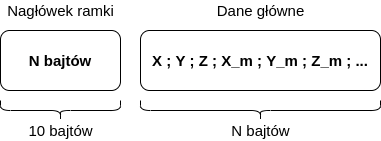
\includegraphics[scale=.5]{ramka}
	\caption{Schemat wiadomości wymienianych pomiędzy urządzeniami. Źródło: [opracowanie własne]} 
	\label{fig:ramka danych}
\end{figure}


\section{Czujniki i kamery}

W celach uproszczenia starano się dobrać czujniki tak aby wszystkie mogły zostać obsłużone przez taki sam interfejs. Do tego celu wybrano magistralę I$^2$C ze względu na jej dużą popularność oraz dostępność różnego rodzaju czujników. Na tę samą magistralę znalezniono również konwerter analogowo-cyfrowy, którego nie posiada domyślnie wybrana platforma. Oprócz czujników komputer obsługuje również dwie kamery, aby uwiecznić postęp wzrostu struktury. Poniżej umieszczono listę modeli wybranych czujników oraz kamer.
\begin{itemize}
	\item Akcelerometr LIS3DH, magistrala I$^2$C
	\item Termometr MCP9808, magistrala I$^2$C
	\item Konwerter analogowo-cyfrowy ADS1115, magistrala I$^2$C
	\item Moduł kamery OV5648, port USB
	
\end{itemize}

Dla czujników przygotowany został osobny moduł \textbf{sensors.py}, który zawiera definicje klas odpowiedzialnych za tworzenie interfejsu między nimi a komputerem komory środowiskowej. Jako, że wszystkie obiekty czujników muszą posiadać metody odpowiedzialne za wysyłanie do nich danych lub ich odbieranie, zostały one oparte o dziedziczenie z abstrakcyjnej klasy bazowej (ang. \angver{abstract base class}, ABC). Oznacza to, iż dzielą one metody o takiej samej nazwie, które docelowo przeznaczone są do tych samych celów, mimo tego iż mogą różnić się zawartością.
\begin{lstlisting}[language=Python, caption={Abstrakcyjna klasa bazowa czujników.}]
class I2CSensor(ABC):

	def __init__(self, address, bus):
		self.address = address
		self.bus = bus
	
	@abstractmethod
	def read(self, *args, **kwargs):
		pass
	
	@abstractmethod
	def enable(self, *args, **kwargs):
		pass
	
	@staticmethod
	@abstractmethod
	def fake_read():
		pass	
\end{lstlisting}
Metody w jakie wyposażono obiekty czujników to wspólny konstruktor \textbf{\_\_init\_\_}, który inicjalizuje obiekt przy okazji przypisując mu otwartą magistralę oraz adres, \textbf{read} zwracającą odczytaną wartość z czujnika, \textbf{enable}, która dokonuje wszystkich operacji koniecznych do poprawnego działania czujnika oraz \textbf{fake\_read}, która emuluje odczyt z czujnika bez konieczności jego podłączenia, co było pomocne w czasie rozwoju programu. Po tak przygotowanej klasie bazowej dziedziczą klasy reprezentujące już konkretne modele czujników, ze względu na różny algorytm odbioru z nich informacji.
\begin{lstlisting}[language=Python, caption={Przykładowa klasa czujnika.}]
class ADS1115ADC(I2CSensor):
	
	__CONVERSION_REG = 0x00
	__CONFIG_REG = 0x01
	__LO_THRESH_REG = 0x02
	__HU_THRESH_REG = 0x03
	
	def read(self, channel):
		# Read channel voltage in reference to ground. ADS1115 also has a differential measuring mode, which
		# has been omitted, but would be trivial to implement.
		
		ls_byte = 0b11100011  # Comparators disabled, 860SPS data rate
		ms_byte = 0b0011 + ((channel + 4) << 4) + 128  # Amplifier gain set to 1, start single conversion, pick channel.
		self.bus.write_i2c_block_data(self.address, ADS1115ADC.__CONFIG_REG, [ms_byte, ls_byte])
		while self.converting_status():
			pass
		data = self.bus.read_i2c_block_data(self.address,ADS1115ADC.__CONVERSION_REG,2)
		reading = (data[0] << 8) + data[1]
		
		return reading
	
	def enable(self):
		pass
	
	@staticmethod
	def fake_read() -> float:
	
		base_read = 50
		
		return float(np.random.normal(base_read, 10, 1))
	
	def converting_status(self):
	
		config = self.bus.read_i2c_block_data(self.address, ADS1115ADC.__CONFIG_REG, 2)
		
		if config[1] >= 128:
			return False
		else:
			return True
\end{lstlisting}

Kamery również obsługiwane są z poziomu programu poprzez wywoływanie poleceń w powłoce systemowej za pomocą biblioteki \textbf{subprocess}. W tym celu przygotowano prosty skrypt \textbf{take\_pic.sh}, który wykonuje zdjęcia za pomocą obu kamer przy użyciu interfejsu Video4Linux. Konieczne jest aby obie kamery posiadały odpowiednie nazwy adapterów portu a, konkretnie \textbf{/dev/videoCam0} oraz \textbf{/dev/videoCam1}. Uzyskiwane jest to za pomocą pliku reguł \textbf{99-name-cameras.rules}, który rozpoznaje unikatowe dla kamer cechy i tworzy odpowiednie dowiązania symboliczne. Plik ten został również umieszczony w repozytorium projektu i należy umieścić go w katalogu \textbf{/etc/udev/rules.d/} w systemie plików komputera komory środowiskowej. Należy zaznaczyć iż numery umieszczone w pliku reguł odpowiadają konkretnym egzamplarzom kamer, a więc jeśli zostaną one zamienione, należy ów kod również zamienić.
\begin{lstlisting}[caption={Plik reguł \textbf{99-name-cameras.rules}.}]
SUBSYSTEM=="video4linux", ENV{ID_REVISION}=="5131",SYMLINK+="videoCam0"
SUBSYSTEM=="video4linux", ENV{ID_REVISION}=="5127",SYMLINK+="videoCam1"
\end{lstlisting}

Na etapie projektu przetestowano kilka dostępnych na rynku czujników wilgotności gleby. Każdy z nich charakteryzował się szybkim postępem korozji elementów wystawionych na działanie wody. Stworzono więc autorski czujnik składający się z dwóch igieł wykonanych ze stali nierdzewnej. Pomiar wilgotności odbywa się poprzez pomiar napięcia układu, w którym układ igieł wbitych w podłoże wzrostowe działa jak rezystor o zmiennym oporze. Aby ograniczyć korozję czujnika do minimum, zasilanie układu jest włączane jedynie na czas pomiaru, trawjący 3s. Na Rys. \ref{fig:czujnik wilg} przedstawiono głowicę wykonanego czujnika wilgotności. Napięcie z układu mierzone jest poprzez dołączony do komputera przetwornik analogowo-cyfrowy. Na Rys. \ref{fig:czujnik wilg sch} widoczny jest prosty schemat elektryczny obwodu czujnika. Zasilanie doprowadzone jest do układu poprzez tranzystor (w tym wypadku jest to fototranzystor zawarty w transoptorze), sterowany z poziomu programu komputera komory środowiskowej. Aby poprawnie interpretować poziomy napięć, konieczny jest pierwszy pomiar napięcia dla głowicy czujnika zanurzonej w wodzie z docelowym stężeniem substancji odżywczych. Dalsze pomiary są następnie przeprowadzane w odniesieniu do tak przygotowanej referencji.

\begin{figure}[h]
	\centering
	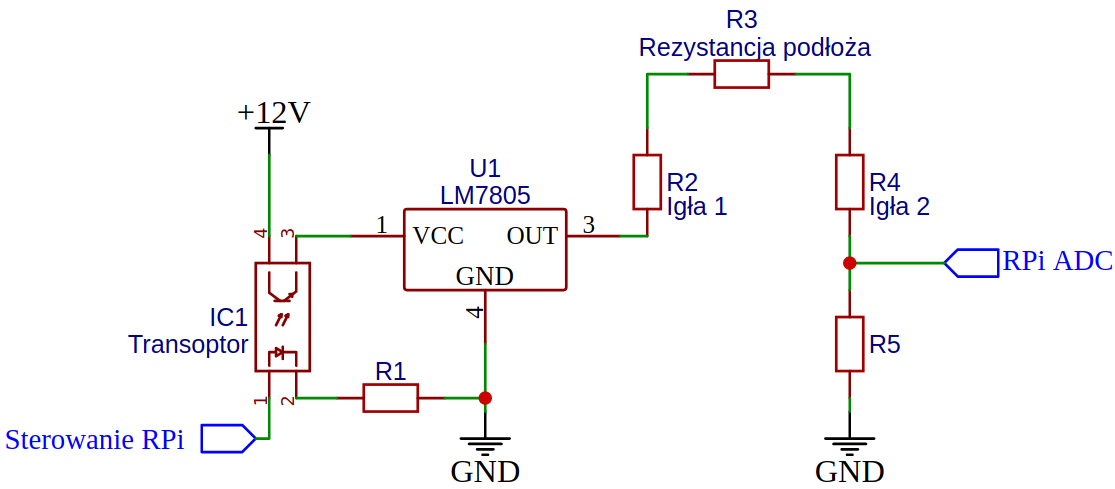
\includegraphics[scale=.4]{schemat_wilg}
	\caption{Schemat elektryczny obwodu czujnika. Źródło: [opracowanie własne]} 
	\label{fig:czujnik wilg sch}
\end{figure}

\begin{figure}[h]
	\centering
	\setlength{\fboxsep}{0pt}
	\setlength{\fboxrule}{1pt}
	\fbox{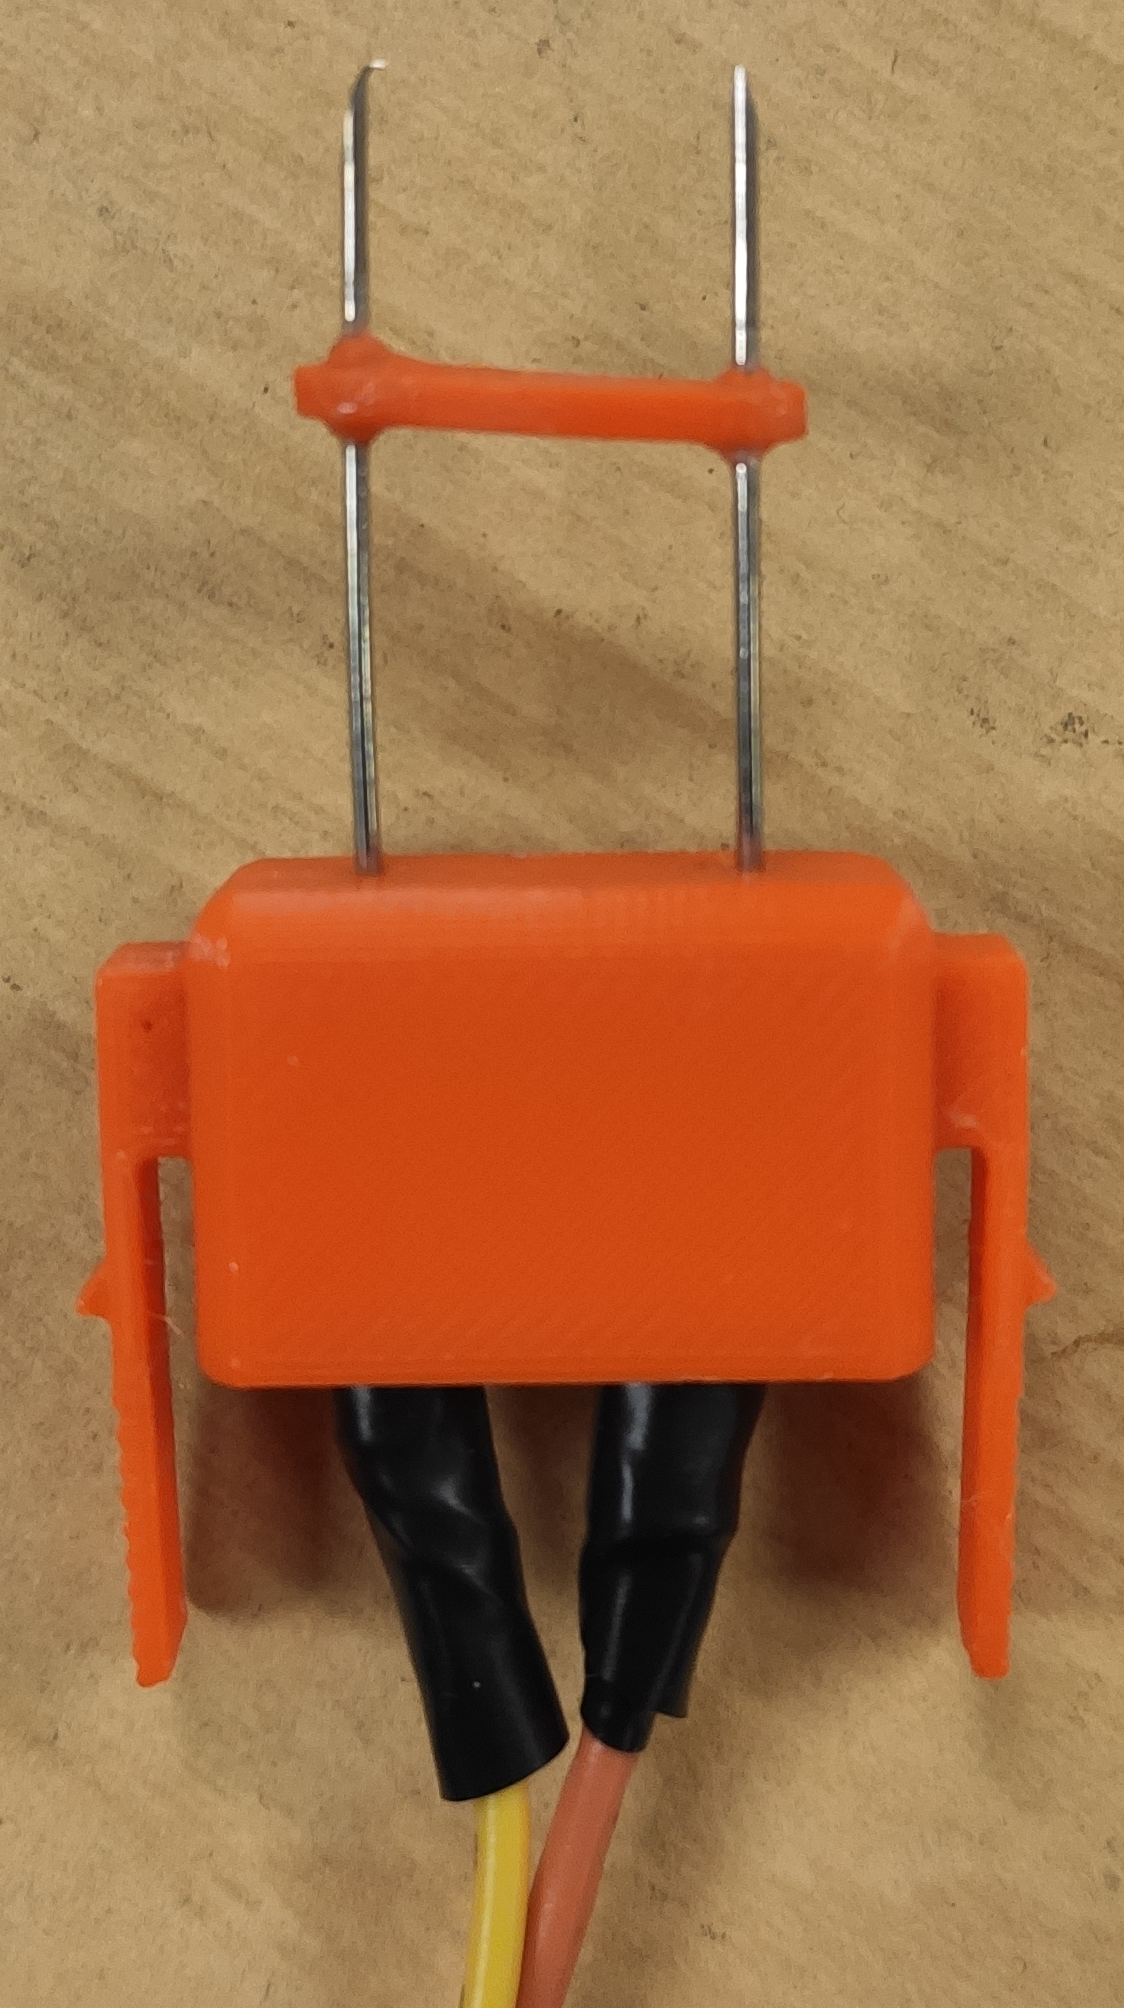
\includegraphics[scale=.15,angle=90]{czujnik_wilg}}
	\caption{Wykonana głowica czujnika wilgotności podłoża. Źródło: [opracowanie własne]} 
	\label{fig:czujnik wilg}
\end{figure}

\chapter{Podsumowanie}

Celem pracy inżynierskiej była budowa systemu kontroli klinostatu w celu umożliwienia przeprowadzania z jego pomocą eksperymentów. W czasie budowy systemu starano się zadbać o jego odporność na działania nieświadomego operatora oraz przejrzystość interfejsu, aby ułatwić jego obsługę. W tym, ostatnim, podsumowującym rozdziale przeprowadzona zostanie ocena stworzonego rozwiązania oraz przedstawione zostaną możliwe ścieżki dalszego jego rozwoju.


\section{Ocena działania systemu}

Stworzony system pozwala na łatwą kontrolę parametrów eksperymentu oraz umożliwia udokumentowanie jego przebiegu w formie danych z czujników oraz zdjęć. Sterowanie samym klinostatem zostało szczegółowo przetestowane przez kilka niezależnych osób, a znalezione błędy zostały naprawione. Daje to dużą pewność co do niezawodności tej części systemu. Przetestowano również każdy moduł stworzony na potrzeby oprogramowania komory środowiskowej, zebrano także pierwsze dane grawitacyjne dla kilkunastominutowych cykli. Zadbano o dokładne testy każdej z części programu komputera komory środowiskowej, co daje pewność odnośnie jego poprawnego działania. Przeprowadzono również testy zkoncentrowane na próbie wymuszenia błędu programu komory z poziomu aplikacji, które zakończyły się pomyślnie. Problemem programu jest czętotliwość z jaką zbierane są dane, ponieważ obecnie wynosi ona \SI{5}{Hz}. Spowodowane jest to głównie kolejkami \textbf{Queue} przez które wymieniane są dane między wątkami. Struktury te są dość powolne i to one ograniczają szybkość wymiany informacji. Drugim elementem jest biblioteka matplotlib, która nie pozwala rozłożyć tworzenia oraz aktualizowania wykresów na kilka wątków. Skutkuje to spowolnieniem wątku głównego kiedy wykresów jest zbyt dużo. Ich obecna ilość została uznana za maksymalną przy której interfejs zachowuje pożądany poziom responsywności pomimo wprowadzenia szeregu optymalizacji.

\section{Perspektywy  dalszego rozwoju systemu}

Pomimo iż stworzony system działa poprawnie oraz spełnia wyznaczone dla niego założenia, istnieje wiele aspektów, w których system mógłby zostać usprawiony lub rozszerzony o dodatkową funkcjonalność. W tym podrozdziale przedstawione zostały moje koncepcje na dalszy rozwój tego oprogramowania.\newline

Obecnie system obsługuje wyłącznie jeden klinostat oraz połączenie tylko z jednym komputerem komory środowiskowej. W przypadku większej ilości urządzeń konieczne byłoby uruchomienie kilku niezależnych instancji tego samego programu, co nie jest dobrym rozwiązaniem. Można więc rozszerzyć go o możliwość obsługi kilku urządzeń jednocześnie, wymagałoby to dodatkowego interfejsu, na którym widoczne byłyby podłączone do systemu urządzenia. W takiej sytuacji należałoby również zrezygnować z komunikacji z klinostatem poprzez port USB, ze względu na ich ograniczoną ilość w każdym komputerze. Rozwiązaniem takie problemu są różnego rodzaju moduły komunikacji bezprzewodowej, które łatwo można obsłużyć poprzez magistrale I$^2$C czy SPI z poziomu MCU klinostatu. Pomimo dużego, pozornego stopnia skomplikowania, rozszerzenie to nie byłoby trudne w implementacji ze względu na obiektową konwencję wykonania obecnego programu. Wymagałoby to natomiast zmiany biblioteki tworzenia wykresów, ze względu na jej ograniczenia wspomniane w podrozdziale \ref{watki}.\\

Kolejnym rozszerzeniem byłby moduł sprzęgający eksperyment kontrolny\linebreak z obecnym eksperymentem przeprowadzanym w klinostacie. Próby kontrolne poddane byłyby dokładnie takim samym warunkom jak główny eksperyment, pomijając klinorotację oraz zewnętrzne warunki magnetyczne. Moduł ten monitorowałby jednocześnie warunki w obu komorach środowiskowych i zapisywał je do jednego pliku. Zmiany ustawień oświetlenia byłyby dzielone przez oba eksperymenty.\\

Do zaprojektowanych przekładni dodano miejsce zamontowania enkoderów obrotowych, co daje możliwość wykrywania kroków gubionych przez silniki oraz dokładne śledzenie pozycji obu stopni swobody klinostatu. Pozwala to na implementację systemu dokładnego pozycjonowania, jeśli pojawi się potrzeba na owy. Nie zdecydowano się go implementować w tej wersji oprogramowania ze względu na to iż nie zostałby on wykorzystany.\\

Teoretycznie system ten również może zostać zaimplementowany do sterowania klinostatmi wysokoobrotowymi, natomiast wymagałoby to kilku, drobnych zmian w kodzie programu. Istnieje możliwość dodania pewnego kroku konfiguracyjnego, zaraz po uruchomieniu programu. Opierałoby się to o poproszenie użytkownika o wprowadzenie parametrów klinostatu takich jak maksymalna prędkość obrotowa, rozdzielczość krokowa silników czy też liczba jednostek napędowych. Program wtedy tworzyłby profil wprowadzonego urządzenia oraz wysłał do sterownika unikatowy identyfikator, który mógłby zostać zapisany w pamięci EEPROM (ang. \angver{Electrically Erasable Programmable Read-Only Memory}) mikrokontrolera. Wczytując wtedy zapisany profil urządzenia, program będzie miał możliwość zidentyfikowania, które urządzenie zostało podłączone. Takie rozwiązanie dałoby możliwość sterowania dowolnym klinostatem, nawet o zupełnie innej konstrukcji bez konieczności ingerowania w kod przez użytkownika.



%%%%%%%%%%%%%%%%%%%%%%%%%%%%%%%%%%%%%%%%%%
\backmatter
\pagenumbering{Roman}
\stepcounter{stronyPozaNumeracja}
\setcounter{page}{\value{stronyPozaNumeracja}}

\pagestyle{tylkoNumeryStron}

%%%%%%%%%%% bibliografia %%%%%%%%%%%%
%\bibliographystyle{plplain}
%\bibliography{Bibliografia/bibliografia}
\printbibliography
\addcontentsline{toc}{chapter}{Bibliografia}
%%%%%%%%%  DODATKI %%%%%%%%%%%%%%%%%%% 

\begin{appendices} 


\chapter*{Dokumentacja techniczna}
\addcontentsline{toc}{chapter}{Dokumentacja techniczna}


\chapter*{Spis skrótów i symboli}
\addcontentsline{toc}{chapter}{Spis skrótów i symboli}

\begin{itemize}
	
	\item[CNC] komputerowe sterowanie numeryczne ({ang. \angver{Computerized Numerical Control}})
	\item[EEPROM] elektrycznie usuwalna i programowalna pamięć tylko do odczytu ({ang. \angver{Electrically Erasable Programmable Read Only Memory}})
	\item[FFM] maszyna spadku swobodnego ({ang. \angver{Free Fall Machine}})
	\item[FRC] klinostat wysoko obrotowy  ({ang. \angver{Fast Rotating Clinostat}})
	\item[HARV] ...  ({ang. \angver{High Aspect Ratio Vessel}})
	\item[LSMM] mikrograwitacja modelowana z zachowaniem niskich naprężeń ścinających w cieczach  (ang. \angver{Low-Shear Modeled Microgravity})
	\item[MCU] mikrokontroler (ang. \angver{Microcontroller Unit})
	\item[PA] poliamid, nylon ({ang. \angver{polyamide}})
	\item[PBL] metoda uczenia przez realizację projektów   ({ang. \angver{Project Based Learning}})
	\item[PETG] politereftalan etylenu domieszkowany glikolem  ({ang. \angver{Polyethylene terephthalate glycol}})
	\item[PP] polipropylen ({ang. \angver{polypropylene}})
	\item[RAM] pamięć dostępu swobodnego ({ang. \angver{Random Access Memory}})
	\item[RPM] maszyna losowego pozycjonowania ({ang. \angver{Random Positioning Machine}})
	\item[RWPV] ...({ang. \angver{Rotating Wall Perfused Vessel}})
	\item[RWV] naczynie z obrotową ścianką  ({ang. \angver{Rotating Wall Vessel}})
	\item[SFR] rejestr specjalnej funkcji ({ang. \angver{Special Function Register}})
	\item[SPI] szeregowy interfejs urządzeń peryferyjnych ({ang. \angver{Serial Peripheral Interface}})
	\item[SRC] klinostat wolno obrotowy ({ang. \angver{Slow Rotating Clinostat}})
	\item[STLV] wolnoobrotowe naczynie boczne  ({ang. \angver{Slow Turning Lateral Vessel}})
	\item[TCP] protokół sterowania transmisją ({ang. \angver{Transmission Control Protocol}})
	\item[TTL] logika tranzysor-tranzystor ({ang. \angver{Transistor-Transistor Logic}})
	\item[USB] uniwersalna magistrala szeregowa ({ang. \angver{Universal Serial Bus}})
	\item[USBASP] szeregowy programator AVR ({ang. \angver{USB AVR serial programmer}})
	\item[UART] uniwersalny asynchroniczny nadajnik odbiornik ({ang. \angver{Universal Asynchronous Receiver Transmiter}})

\end{itemize}



\chapter*{Zawartość dołączonej płyty}
\addcontentsline{toc}{chapter}{Zawartość dołączonej płyty}

Do pracy dołączona jest płyta CD z~następującą zawartością:
\begin{itemize}
\item praca w~formacie \texttt{pdf},
\item źródła programu,
\item zbiory danych użyte w~eksperymentach.
\end{itemize}

\listoffigures
\addcontentsline{toc}{chapter}{Spis rysunkow}
\listoftables
\addcontentsline{toc}{chapter}{Spis tabel}
	
\end{appendices}


\end{document}


%% Finis coronat opus.
